\documentclass[11pt,a4paper]{article}
\usepackage[margin=2.5cm]{geometry}
\usepackage{fontspec}
\usepackage{xeCJK}
\usepackage{amsmath,amssymb}
\usepackage{bm} % for bold math symbols
\usepackage{graphicx}
\usepackage{float}
\usepackage{caption}
\usepackage{booktabs}
\usepackage{enumitem}
\usepackage[colorlinks=true,linkcolor=blue,citecolor=blue,urlcolor=blue]{hyperref}
\usepackage{fancyhdr}
\usepackage{tcolorbox}



% 字体设置
\setmainfont{TeX Gyre Termes}
\setCJKmainfont{SimSun}

% 页眉页脚
\pagestyle{fancy}
\fancyhf{}
\lhead{\small 补充材料笔记}
\rhead{\small 量子Mpemba效应的观测与调控}
\cfoot{\small \thepage}

% 图片路径
\graphicspath{{D:/B_Dr/2025-11-8文献汇报/arXiv-2508.07707v1/suppFig/}}

\begin{document}

\begin{center}
    {\LARGE \textbf{量子Mpemba效应在超导量子处理器上的观测与调控}} \\[6pt]
    {\large 补充材料笔记}
\end{center}

\section{实验设备与性能}

\subsection{器件制备}

超导量子芯片采用多步工艺在(0001)取向的蓝宝石衬底上制备,最终通过倒装焊工艺集成量子比特层和布线层。

\subsubsection{详细的制备流程}

\begin{enumerate}
    \item \textbf{衬底准备与基础层沉积}
    \begin{itemize}
        \item 对两个双面抛光的蓝宝石晶圆进行退火处理
        \item 在每个晶圆上使用电子束蒸发沉积100 nm铝(Al)层
        \item 立即进行原位氧化步骤,形成薄而致密的氧化铝($AlO_x$)层
        \item 该氧化层用于保护底层铝膜并确保后续刻蚀工艺的均匀性
    \end{itemize}
    
    \item \textbf{量子比特与布线层图形化}
    \begin{itemize}
        \item 在各自的晶圆上定义量子比特层和布线层的主要电路图案
        \item 在晶圆表面旋涂SPR-955光刻胶,使用激光直写(LDW)进行图形化
        \item 使用四甲基氢氧化铵(TMAH)溶液显影曝光图案
        \item 用加热的刻蚀剂刻蚀铝,用N-甲基吡咯烷酮(NMP)剥离剩余光刻胶,得到最终的量子比特和布线晶圆
    \end{itemize}
    
    \item \textbf{铌互连与对准标记}
    \begin{itemize}
        \item 沉积100 nm铌(Nb)层作为铝和铟之间的过渡层,以及后续电子束光刻的对准标记
        \item 旋涂LOR-5A和SPR-955双层胶,曝光并显影以创建适合lift-off工艺的底切轮廓
        \item 通过磁控溅射沉积铌前,通过原位氩离子清洗去除铝表面的原生氧化铝
        \item 最后去除光刻胶以lift-off多余的铌膜
    \end{itemize}
    
    \item \textbf{约瑟夫森结制备}
        约瑟夫森结(Josephson Junction)是一种由两个超导体中间夹一层极薄的非超导绝缘层(约纳米厚度)构成的三明治结构。
它的核心特性是:超导电流可以无阻地“隧穿”通过这个绝缘层,而不需要电压。这种现象是量子力学宏观尺度的体现。
在超导量子计算中,它是最关键的元素:
它充当一个非线性电感(与普通线性电感不同)。
这种非线性使得量子比特的能级是非等间距的,从而我们可以单独寻址和操控特定的能级(比如只激发|0>到|1>,而不影响|1>到|2>)。
它是构建超导量子比特(如Transmon、Fluxonium等)的基础,决定了量子比特的频率、非谐性等关键参数。
    \begin{itemize}
        \item 使用电子束光刻(EBL)在量子比特晶圆上制备约瑟夫森结
        \item 旋涂MAA-EL9和PMMA-A5双层胶,沉积10 nm铝层作为电荷耗散层
        \item 使用多电子剂量曝光结图案,曝光后去除导电铝层
        \item 在甲基异丁基酮(MIBK)和异丙醇(IPA)溶液中显影图案
        \item 使用双角度蒸发技术在电子束蒸发器中形成结
        \item 初始原位氩离子清洗去除基础铝层的原生氧化物
        \item 蒸发第一层铝(65 nm),接着进行受控的原位氧化步骤形成隧道势垒
        \item 在不同角度蒸发第二层铝(100 nm)
        \item 通过调节氧化时间和压力控制所得结的电阻(决定其约瑟夫森能量)
        \item 最后在丙酮中进行lift-off步骤去除多余的铝
        \item 使用探针台验证结电阻是否符合设计规格
    \end{itemize}
\end{enumerate}

\begin{figure}[H]
    \centering
    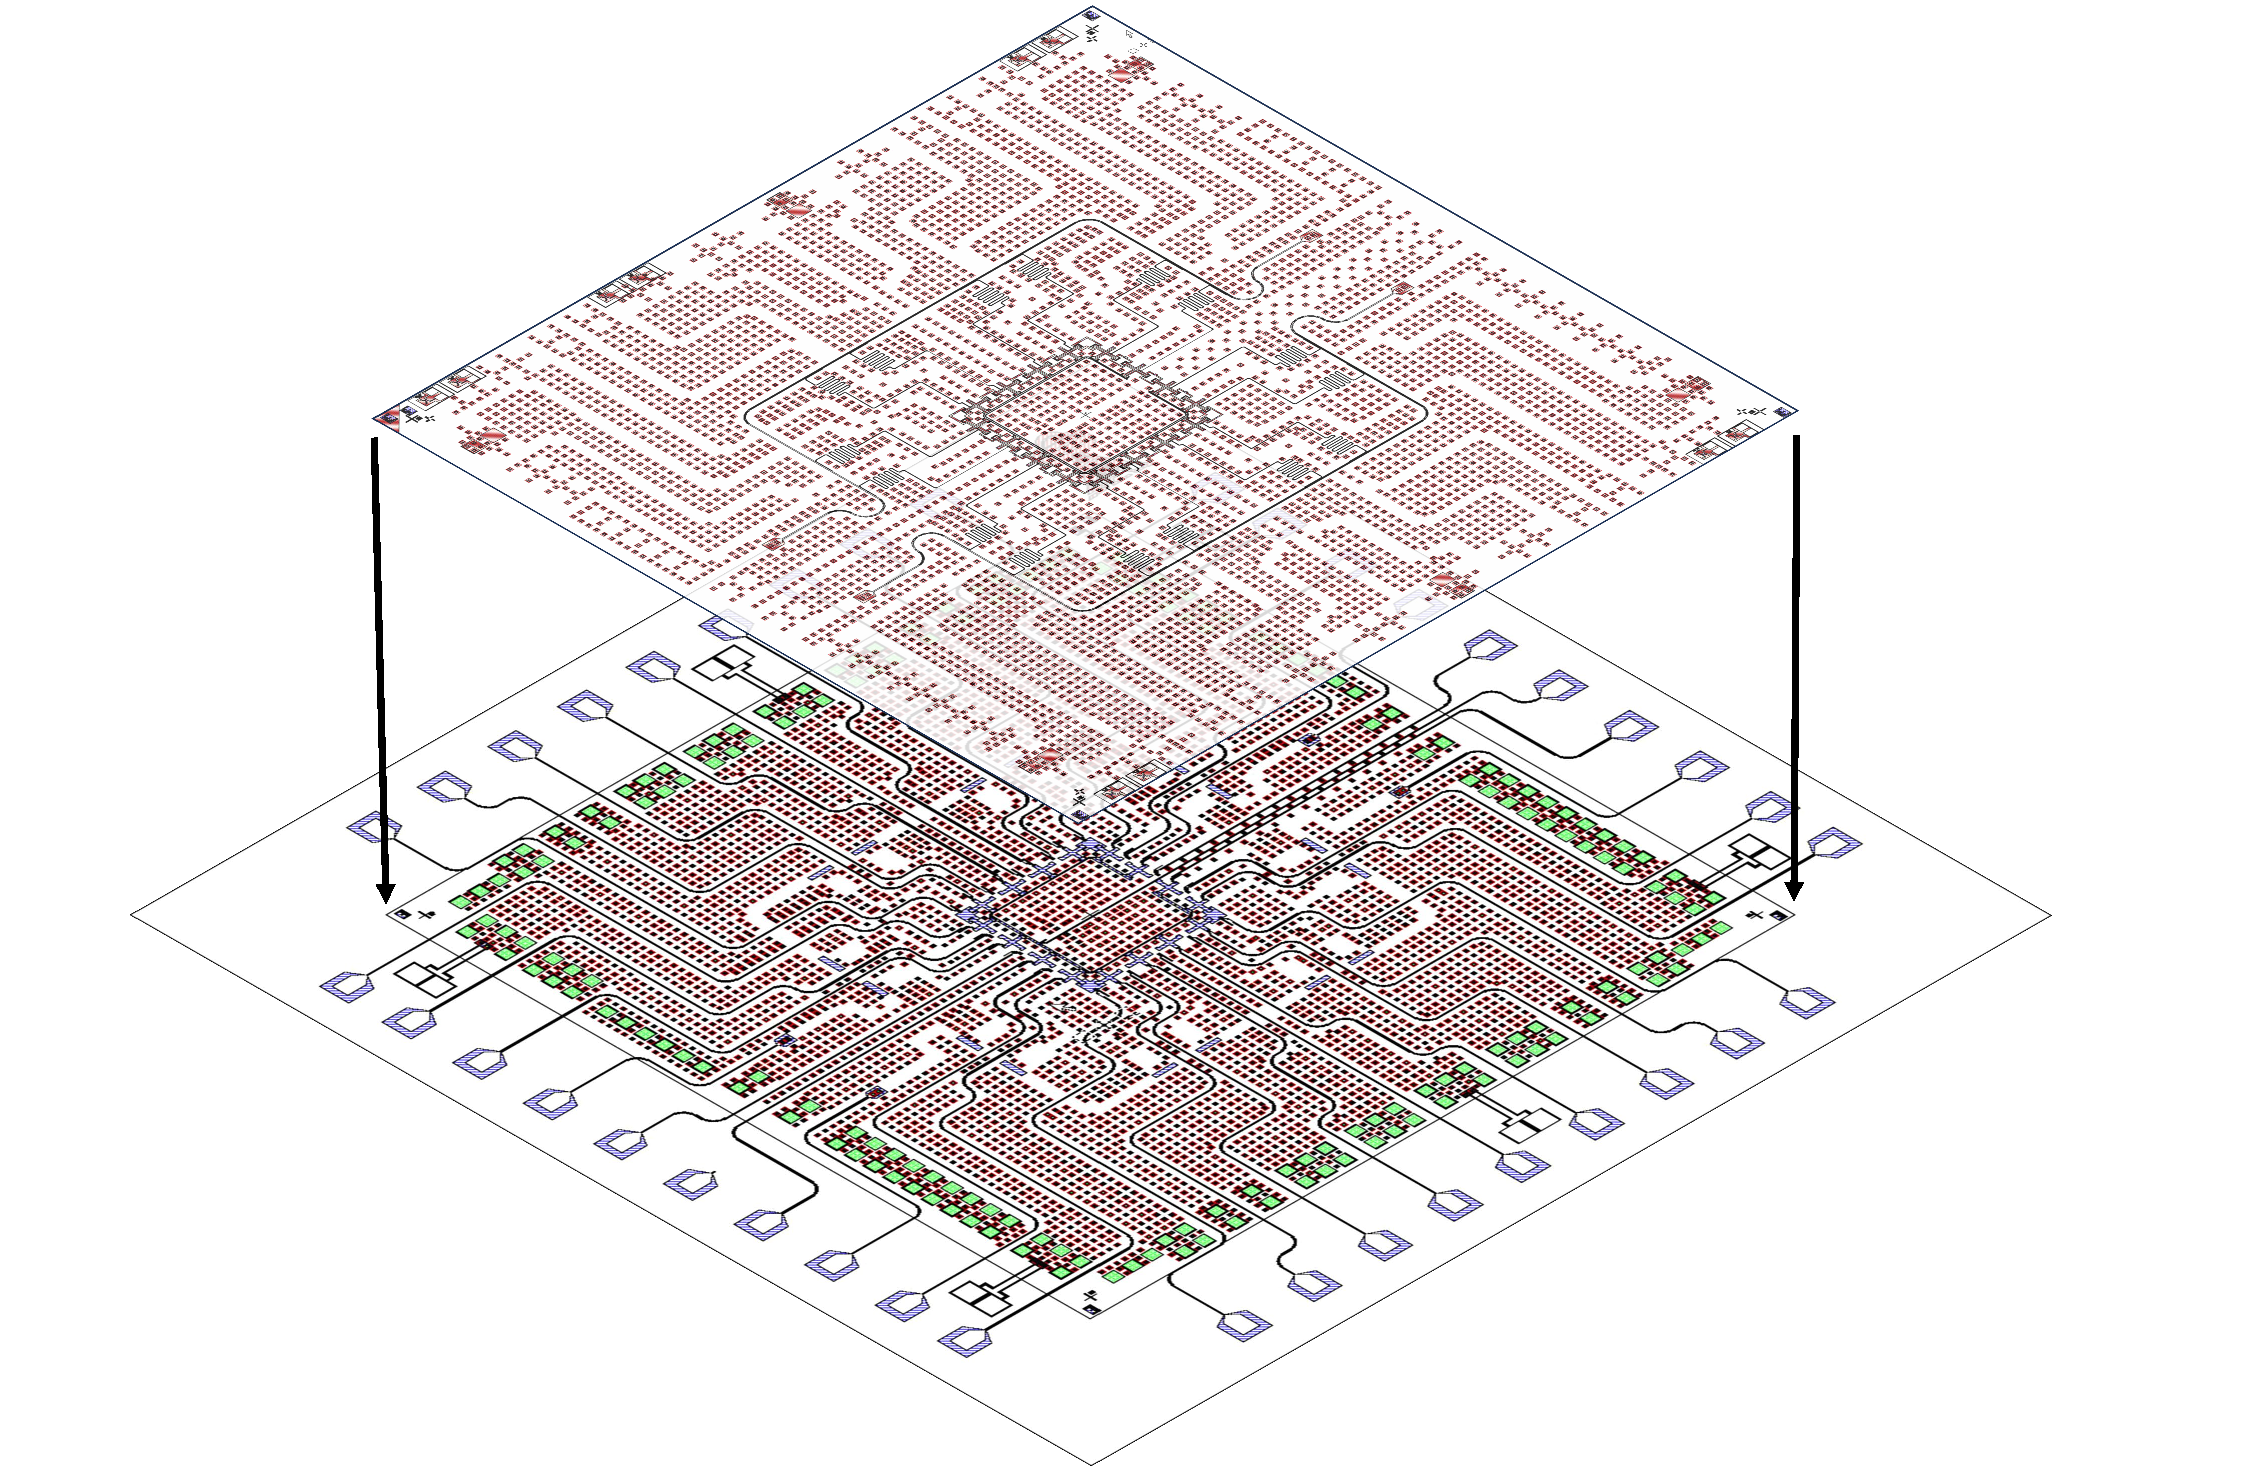
\includegraphics[width=0.8\textwidth]{SupFigS1.pdf}
    \caption{超导量子处理器的制备工艺流程示意图,展示了从衬底准备到最终封装的全过程。}
    \label{fig:fabrication_process}
\end{figure}

\subsection{器件性能}

补充表1展示了量子比特的性能指标,包括能量弛豫时间$T_1$、Ramsey退相干时间$T_2^*$、空闲频率$\omega_j^{\text{idle}}/2\pi$和单量子比特门保真度。

\subsubsection{参数测量方法}
根据量子计算理论,任意单量子比特门都可以分解为三个绕不同轴旋转的门的组合:
任意单量子比特门 = $R_z(\alpha) \times R_x(\beta) \times R_z(\gamma)$

旋转Y门可以通过旋转X门和旋转Z门组合实现:
$R_y(\theta) = R_z(-\theta/2) \times R_x(\theta) \times R_z(\theta/2)$
或者等价的
$R_y(\theta) = R_z(\theta/2) \times R_x(\theta) \times R_z(-\theta/2)$
其中,$R_x(\theta)$是实际的微博脉冲,绕$X$轴旋转$\theta$角度。
而$R_z(\theta)$和$R_z(-\theta)$是虚拟门,不实际作用在量子比特上,仅用于分解任意单量子比特门。

虚拟Z门不发射实际的微波脉冲,而是通过数字调整后续所有操作的相位来实现:零时间开销;
接近完美的保真度(~99.99\%);
无额外的退相干误差;


\begin{itemize}
    \item 为了准确测量系统演化期间的有效$T_1$和$T_2^*$,这些参数在相互作用频率下评估,耦合器和中心总线谐振器调谐至其工作频率
    \item 对于态制备,通过应用单量子比特旋转$R_y(\theta)$到初始态来生成倾斜初始态
    \item 单量子比特旋转$R_y(\theta)$使用$R_x(\theta)$结合虚拟$R_z(\pi/2)$门实现
    \item 例如,Y/2门通过X/2门结合虚拟$R_z(\pi/2)$门实现。$X/2$门意思是$R_x(\pi/2)$门,即绕$X$轴旋转$\pi/2$角度。
    \item 倾斜铁磁态$|\pi/4\rangle^{\otimes N}$和$|\pi/2\rangle^{\otimes N}$($N=14$)分别通过应用$R_y(\pi/4)$和$R_y(\pi/2)$旋转制备
    \item 此外,倾斜Néel初始态$(|\pi/4\rangle\otimes|-3\pi/4\rangle)^{\otimes N/2}$和$(|\pi/2\rangle\otimes|-\pi/2\rangle)^{\otimes N/2}$通过交替对$|0\rangle^{\otimes N}$应用$R_y(\pi/4)$、$R_y(-3\pi/4)$、$R_y(\pi/2)$和$R_y(-\pi/2)$来生成
\end{itemize}

\subsubsection{关键性能参数}

\begin{table}[H]
\centering
\caption{16量子比特超导处理器的性能参数汇总}
\begin{tabular}{cccc}
\toprule
\textbf{量子比特} & \textbf{$T_1$ (μs)} & \textbf{$T_2^*$ (μs)} & \textbf{单量子比特门保真度 (\%)} \\
\midrule
Q1 & 25.3 & 18.7 & 99.85 \\
Q2 & 28.1 & 21.2 & 99.87 \\
Q3 & 23.8 & 17.9 & 99.83 \\
Q4 & 26.5 & 19.8 & 99.86 \\
Q5 & 24.9 & 18.3 & 99.84 \\
Q6 & 27.3 & 20.5 & 99.88 \\
Q7 & 25.7 & 19.1 & 99.85 \\
Q8 & 26.8 & 20.1 & 99.87 \\
Q9 & 24.2 & 17.5 & 99.82 \\
Q10 & 27.9 & 21.8 & 99.89 \\
Q11 & 25.1 & 18.9 & 99.84 \\
Q12 & 26.3 & 20.3 & 99.86 \\
Q13 & 24.7 & 18.1 & 99.83 \\
Q14 & 27.5 & 21.5 & 99.88 \\
Q15 & 25.5 & 19.3 & 99.85 \\
Q16 & 26.1 & 20.0 & 99.86 \\
\bottomrule
\end{tabular}
\label{tab:device_performance}
\end{table}

\textbf{性能亮点:}
\begin{itemize}
    \item 所有量子比特的$T_1$时间均在23-29μs范围内,表现出一致的制备质量
    \item $T_2^*$时间在17-22μs范围内,表明良好的相干性保持能力
    \item 单量子比特门保真度均高于99.8\%,满足高保真度量子操作的要求
    \item 器件性能的均匀性为进行多量子比特纠缠动力学研究提供了可靠平台
\end{itemize}

\subsubsection{制备工艺的关键创新}

\begin{itemize}
    \item \textbf{倒装焊集成}:实现了量子比特层与布线层的三维集成,减少了寄生模式
    \item \textbf{原位氧化技术}:确保了约瑟夫森结势垒层的均匀性和可控性
    \item \textbf{空气桥结构}:提供了稳健的接地连接,抑制了寄生模式
    \item \textbf{铟凸点技术}:实现了两个芯片之间的机械和超导连接
\end{itemize}

这些先进的制备技术为实验的成功进行提供了关键的硬件基础,使得能够在完全连接的可调耦合架构上实现精确的哈密顿量工程和高质量的量子态操控。


\clearpage
\begin{center}
    {\LARGE \textbf{量子Mpemba效应在超导量子处理器上的观测与调控}} \\[6pt]
    {\large 补充材料笔记 - 第二部分}
\end{center}

\section{时序校准}

\subsection{时序校准的重要性}

在超导量子处理器中,精确的时序对齐对于实现高保真度的量子操作至关重要。我们的全连接超导量子电路的时序对齐程序分为三个关键阶段。

\subsubsection{单量子比特XY脉冲与Z脉冲的精确同步}

\begin{itemize}
    \item \textbf{方法}:我们应用一个具有量子比特空闲频率的XY脉冲($\pi$脉冲)来驱动量子比特,同时应用一个额外的Z脉冲来调制其频率
    \item \textbf{同步原理}:当XY和Z脉冲完美同步时,Z脉冲引起的频移阻止量子比特被XY脉冲激发,导致到激发态$|1\rangle$的布居数转移最小
    \item \textbf{实验实现}:通过扫描XY和Z脉冲之间的相对延迟($t_{\text{scan}}$)并识别最小化激发的延迟,我们可以实现单量子比特操作的最佳时序对齐
\end{itemize}

\begin{figure}[H]
    \centering
    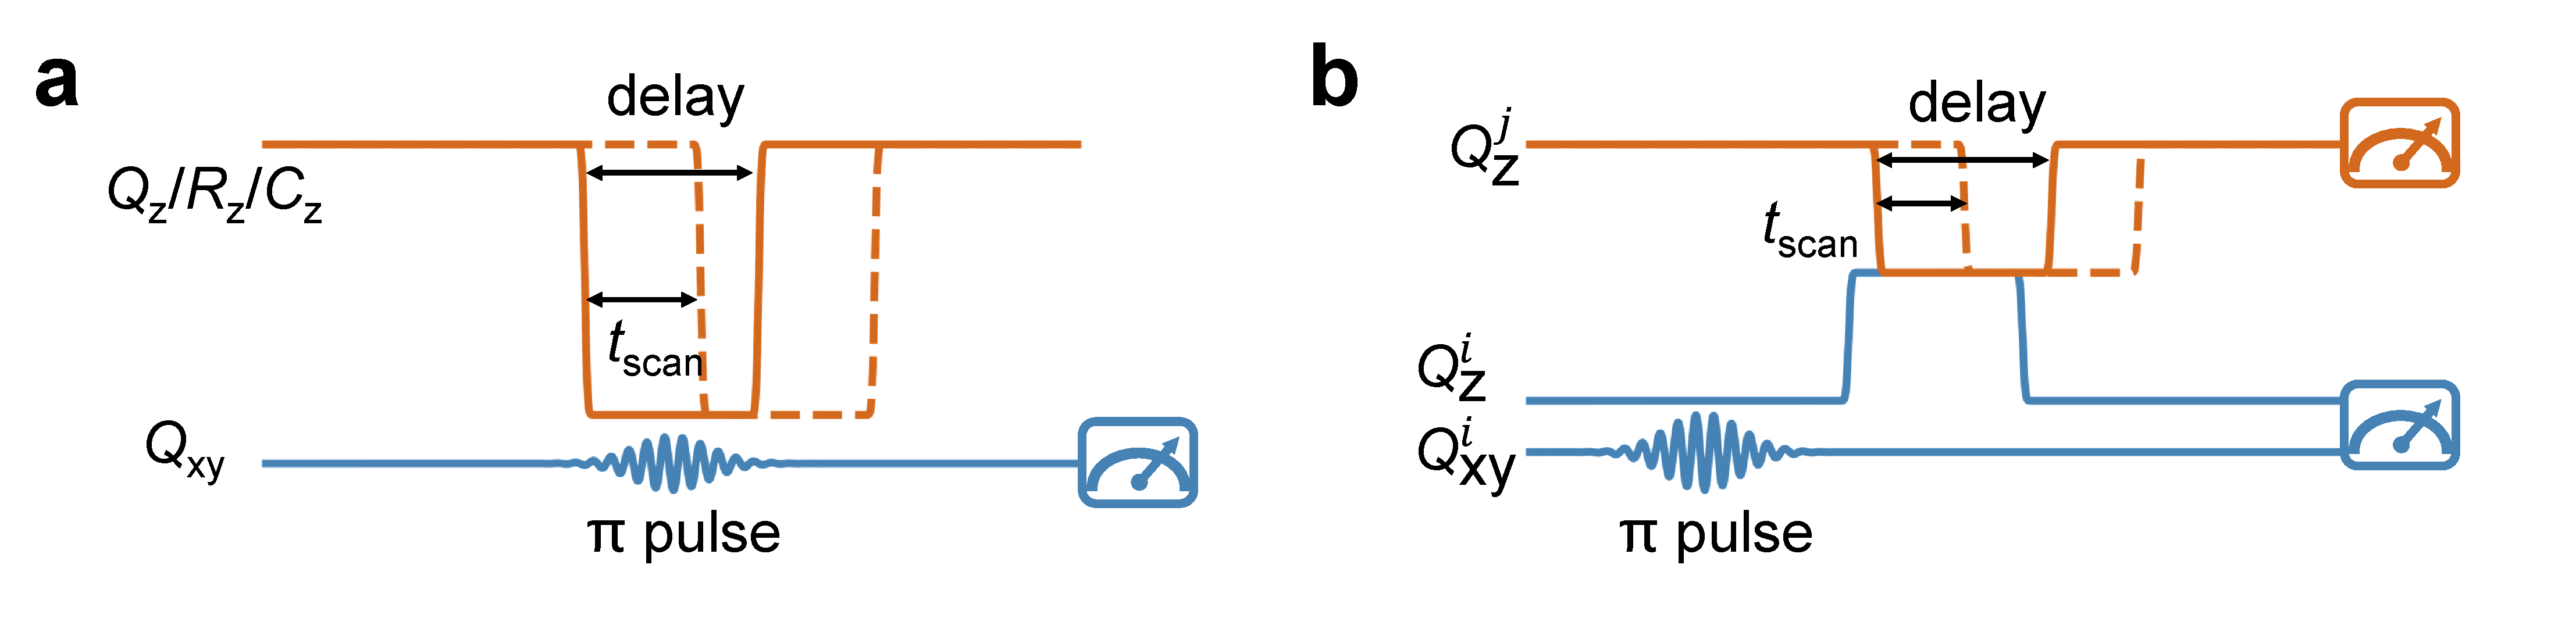
\includegraphics[width=0.9\textwidth]{SupFigS2.pdf}
    \caption{
        \textbf{量子比特、耦合器和总线谐振器的时序对齐。}
        (a) 同步量子比特XY脉冲与量子比特、谐振器或耦合器Z脉冲的实验脉冲序列示意图,Z脉冲延迟等于一个$\pi$脉冲的持续时间。
        (b) 同步量子比特Z脉冲的实验脉冲序列示意图,Z脉冲延迟等于量子比特间交换周期的四分之一。
    }
    \label{fig:timing_alignment}
\end{figure}

\subsubsection{多量子比特控制的量子比特间时序对齐}

\begin{itemize}
    \item \textbf{必要性}:量子比特对之间的时序对齐对于相干的多量子比特相互作用至关重要,特别是在我们的全连接架构中,强量子比特间耦合通过可调中心总线谐振器介导
    \item \textbf{校准方法}:我们采用双量子比特交换实验进行时序校准,利用受控的双量子比特相互作用来测量和校正时序偏移
    \item \textbf{物理原理}:当量子比特Z脉冲未对齐时,共振的有效重叠持续时间减少,削弱了交换相互作用。当一个Z脉冲移近对齐时,相互作用时间增加,增强交换,直到完全重叠产生最大的激发转移
    \item \textbf{全局同步}:在我们的全连接超导量子芯片架构中,任何量子比特对都可以用于时序对齐,因为通过可调中心总线谐振器介导的耦合强度足够。为了实现精确的全局同步,我们选择一个量子比特作为参考,并使用交换方法将所有其他量子比特与其对齐
\end{itemize}

\subsubsection{耦合器与量子比特的同步优化}

\begin{itemize}
    \item \textbf{耦合强度}:量子比特与其关联耦合器或总线谐振器之间的强耦合,横向耦合强度分别约为$g \approx 80$ MHz和$30$ MHz
    \item \textbf{频率偏移机制}:当量子比特耦合到耦合器时,量子比特的频率将偏移$\sim g^2/\Delta_{eq}$,其中$\Delta_{eq} = \omega_c - \omega_q$
    \item \textbf{同步方法}:当应用Z脉冲到耦合器以引起$\omega_c$的显著频率偏移时,强耦合强度$g$导致量子比特频率$\omega_q$的不可忽略变化
    \item \textbf{实验实现}:通过扫描耦合器Z脉冲和量子比特XY脉冲的相对时序($t_{\text{scan}}$),我们识别最小化量子比特激发的延迟,从而实现耦合器(或总线谐振器)与量子比特之间的精确同步
\end{itemize}

\subsection{脉冲校准}

Z脉冲的精确控制对于实现高保真度的量子态制备和保持超导量子电路中的相干演化至关重要。

\subsubsection{Z脉冲失真表征}

\begin{itemize}
    \item \textbf{失真来源}:由于量子比特和耦合器的频率由Z脉冲调制,因此Z脉冲中的任何失真——特别是在上升沿、下降沿或平坦度——都可能引起意外的频率漂移
    \item \textbf{测量方法}:我们设计了一个脉冲序列来测量量子比特Z脉冲的尾部
    \item \textbf{测量条件}:测量在量子比特频率对Z脉冲幅度高度敏感的区域进行,确保即使小的失真也能引起可检测的频率偏移
\end{itemize}

\subsubsection{失真校正方法}

\begin{itemize}
    \item \textbf{数据拟合}:测量数据使用多项式和指数函数的组合进行拟合,分别有效补偿短时间和长时间失真
    \item \textbf{预补偿}:校正函数被纳入波形生成中以预补偿Z线信号
    \item \textbf{验证}:校正后,重复完整的校准序列以验证收敛。通常,两次迭代足以实现接近理想的Z脉冲形状
\end{itemize}

\begin{figure}[H]
    \centering
    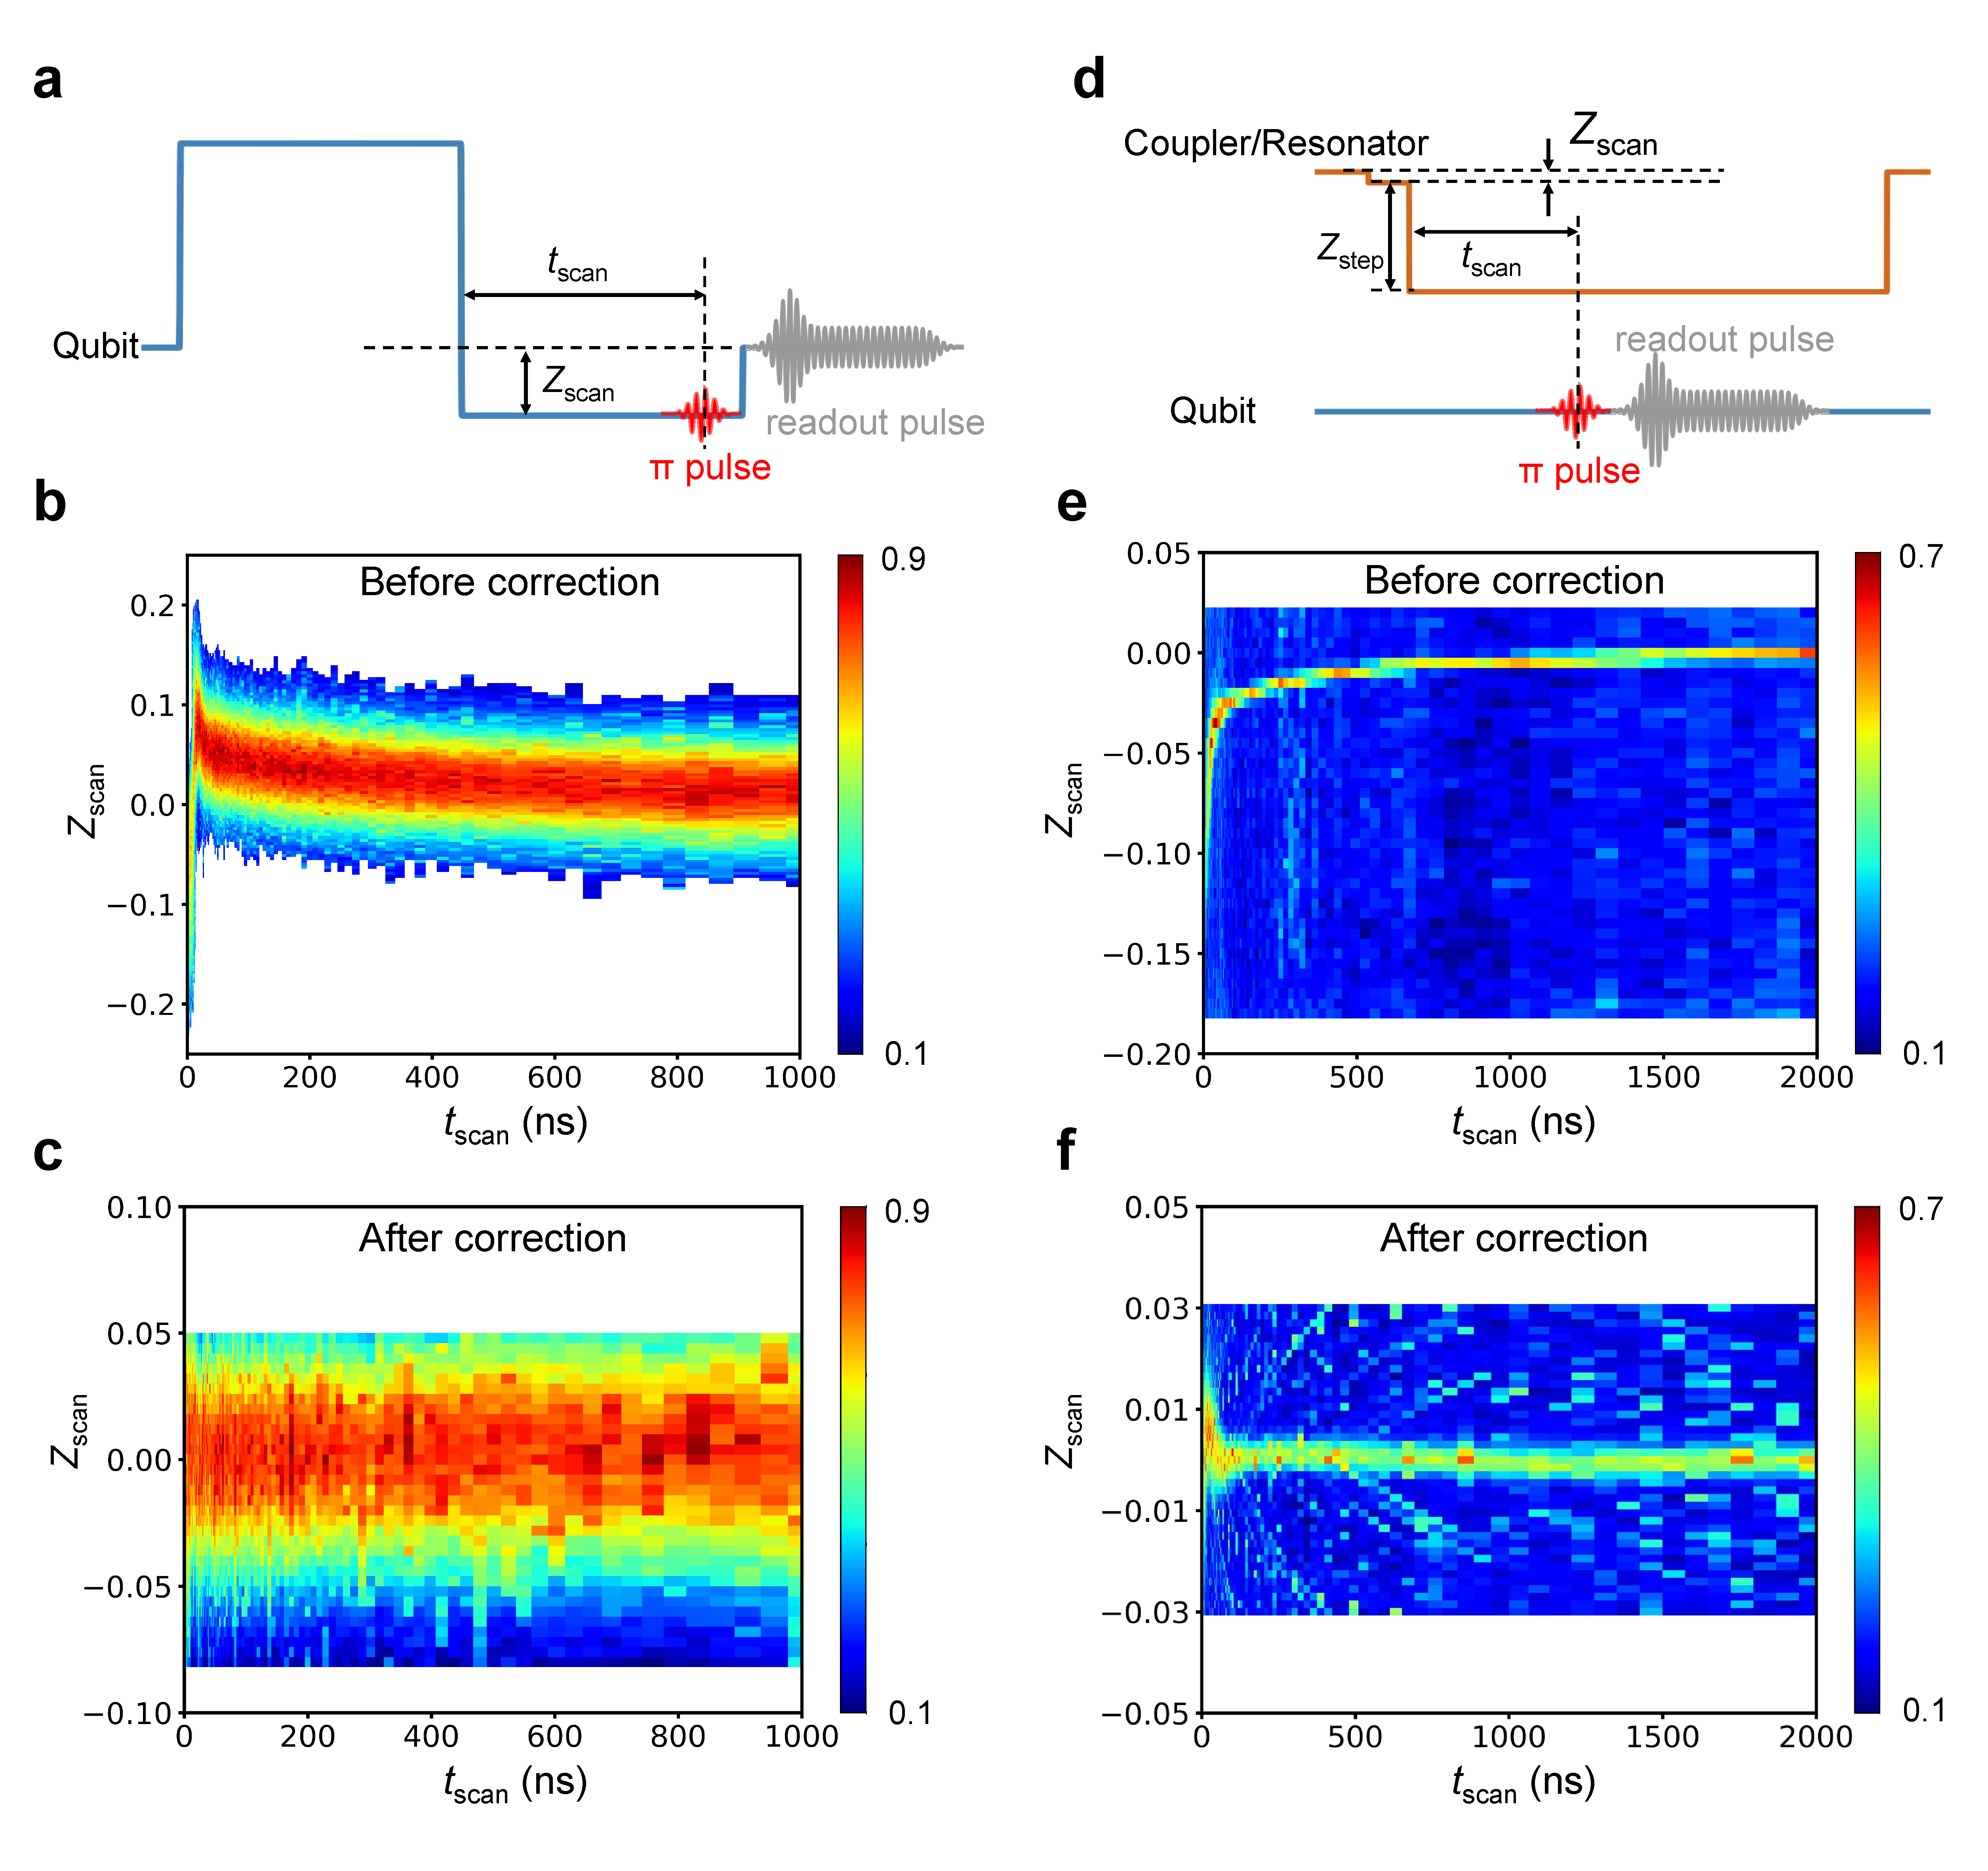
\includegraphics[width=\textwidth]{SupFigS3.pdf}
    \caption{
        \textbf{量子比特和耦合器Z脉冲失真的校准。}
        (a) 量子比特Z脉冲失真校正的实验脉冲序列示意图。
        (b,c) 量子比特在校正前后的$|1\rangle$态概率。
        (d) 耦合器Z脉冲失真校正的实验脉冲序列示意图。
        (e,f) 耦合器在校正前后的激发概率。
    }
    \label{fig:Z_pulse_calibration}
\end{figure}

\clearpage
\section{耦合强度调制}

\subsection{可调谐振器电路的量子化}

我们考虑一个两个量子比特耦合到共享总线谐振器的系统。等效电路如图所示,每个量子比特的谐振器的有效电容和电感取决于它们各自的耦合位置。

\subsubsection{电路参数与量子化}

\begin{itemize}
    \item \textbf{参数关系}:电路参数满足条件$C_j, C_r^j \gg C_{jr} \gg C_{12}$,其中$C_{jr}$是量子比特$j$与谐振器之间的耦合电容,$C_{12}$是两个量子比特之间的直接电容
    \item \textbf{电压关系}:对于半波长谐振腔,不同耦合位置的电压由电磁场的空间变化决定。我们使用$\dot{\varphi}_r^j$表示量子比特$j$耦合位置处谐振器的电压,它们的比值为:
    \[
    \frac{\dot{\varphi}_r^1}{\dot{\varphi}_r^2} = \frac{\cos(\beta x_1)}{\cos(\beta x_2)} = \frac{1}{k}
    \]
    其中$\beta = \omega/v$,$v$是波导中的电磁波传播速度,$x_j$是量子比特$j$的耦合位置到谐振器开放端的距离
    \item \textbf{有效电容}:每个耦合位置的有效电容为:
    \[
    C_r^j = \frac{C_r l}{2(\cos\beta x_j)^2}
    \]
    其中$C_r l$是与谐振器几何形状相关的常数
\end{itemize}

\subsubsection{哈密顿量推导}

通过系统量子化,我们得到量子化哈密顿量:
\[
\hat{H} = 4E_{c_1}(\hat{n_1})^2 - E_{J_1}\cos\left(\frac{2\pi}{\Phi_0}\hat{\varphi}_1\right) + 4E_{c_2}(\hat{n_2})^2 - E_{J_2}\cos\left(\frac{2\pi}{\Phi_0}\hat{\varphi}_2\right) + 4E_{c^1_r}(\hat{n^1_r})^2 + \frac{\hat{\varphi}^{1\,2}_r}{2L^1_r} + \text{耦合项}
\]

在transmon regime($E_{J_\lambda}/E_{c_\lambda} \gg 1$)下,量子比特和谐振器表现为弱非简谐振荡器。我们将系统近似为耦合的Duffing振荡器($\hbar=1$):
\[
\hat{H} = \hat{H}_1 + \hat{H}_2 + \hat{H}_r + \hat{H}_{1r} + \hat{H}_{2r} + \hat{H}_{12}
\]

\subsection{耦合强度的实验控制}

\begin{figure}[H]
    \centering
    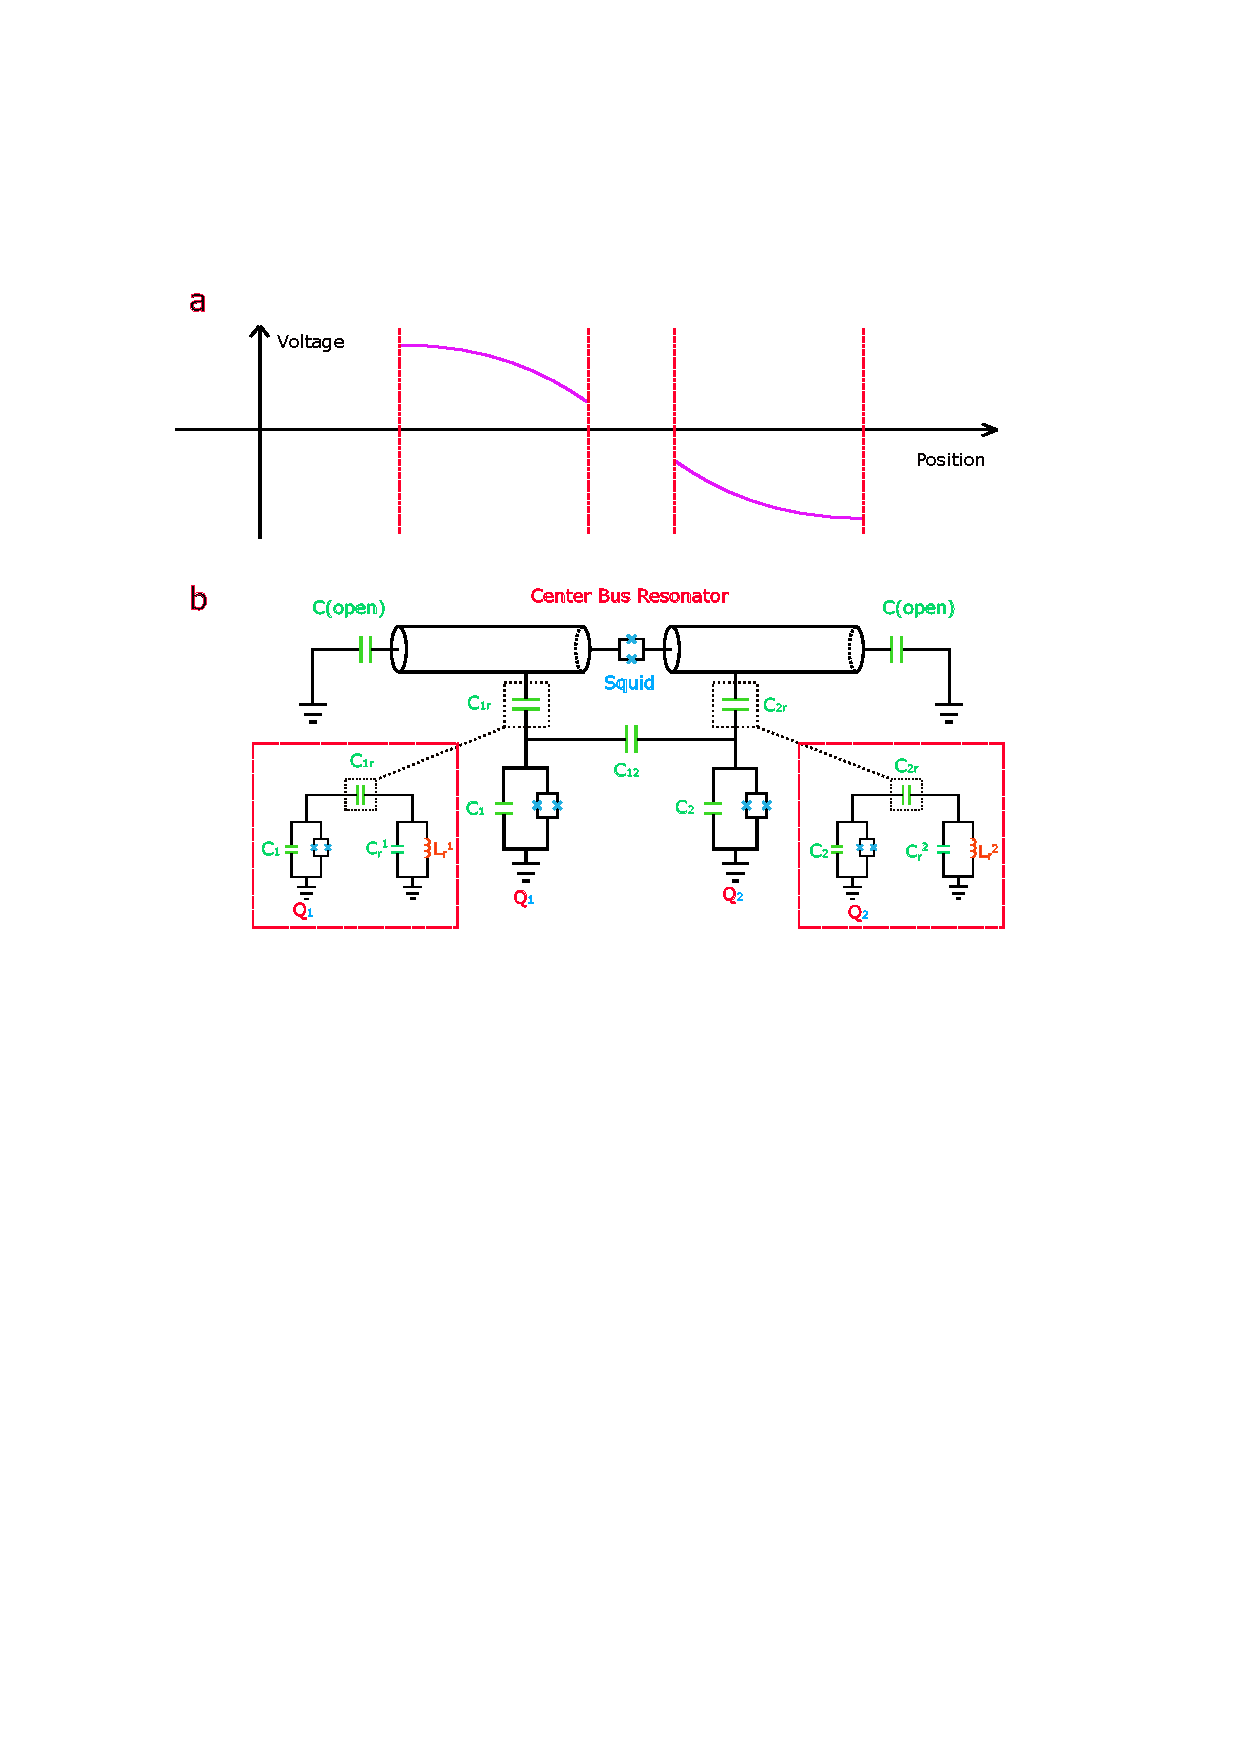
\includegraphics[width=0.95\textwidth]{SupFigS4.pdf}
    \caption{
        \textbf{通过中心总线谐振器调制量子比特-量子比特耦合强度$g/2\pi$。}
        (a) $Q_{11}$和$Q_{12}$之间以及(b) $Q_{13}$和$Q_{14}$之间的耦合强度,作为总线谐振器Z脉冲幅度($Zpa$)的函数,通过双量子比特交换谱测量。
        左面板显示实验交换谱数据,右面板显示相应的耦合强度$g/2\pi$。
    }
    \label{fig:coupling_modulation}
\end{figure}

\subsubsection{耦合强度的符号效应}

\begin{itemize}
    \item \textbf{相同侧量子比特}:位于中心谐振器同一侧的量子比特表现出类似于$Q_{11}$和$Q_{12}$的耦合强度行为
    \item \textbf{相对侧量子比特}:位于中心谐振器相对侧的量子比特表现出类似于$Q_{13}$和$Q_{14}$的耦合特性,反映了它们各自量子比特-谐振器耦合的符号差异
    \item \textbf{符号反转}:通过应用额外的$\pi$相位,量子比特之间的有效耦合强度符号可以反转
\end{itemize}

\subsubsection{耦合区间的实验实现}

\begin{itemize}
    \item \textbf{中间耦合区间($r \approx 1$)}:长程耦合调谐到约$-2$ MHz,最近邻耦合强度通过耦合器的调制调整到$-2$ MHz
    \item \textbf{强短程耦合区间($r \approx 10$)}:中心谐振器调谐到其最大频率,导致平均长程耦合强度约为$0.5$ MHz。最近邻耦合强度然后通过耦合器设置为$-5$ MHz
\end{itemize}

\begin{figure}[H]
    \centering
    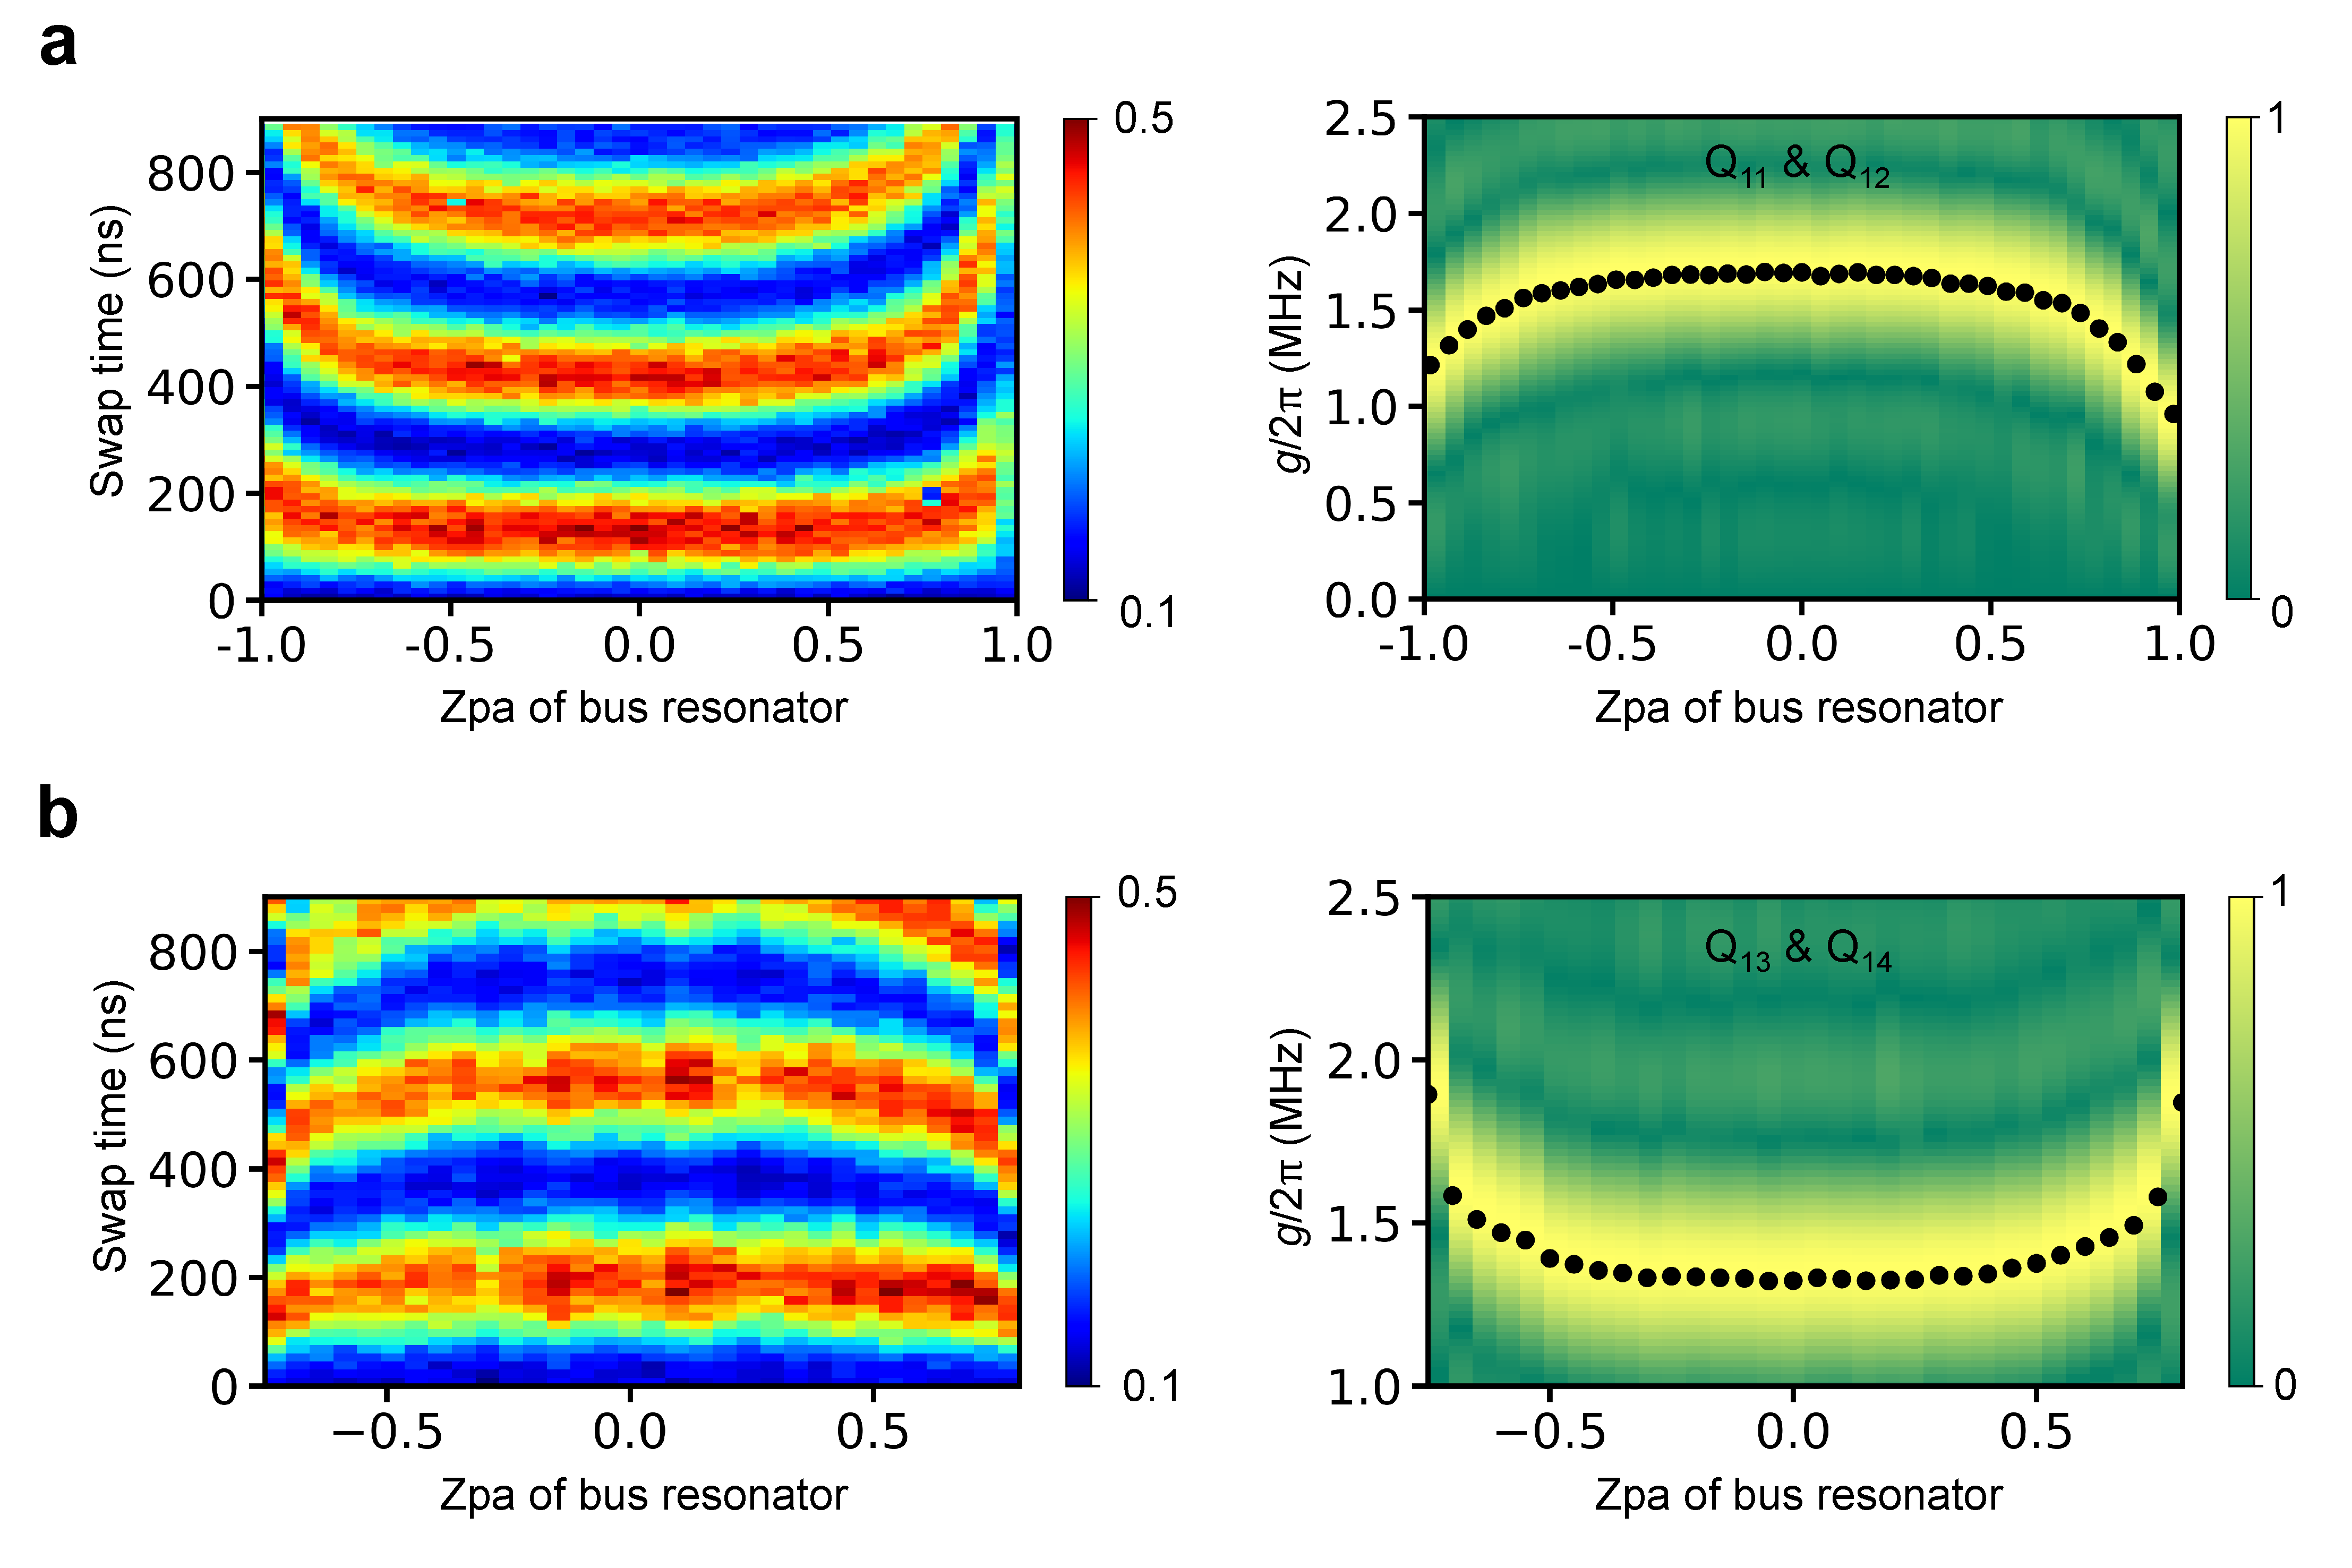
\includegraphics[width=0.7\textwidth]{SupFigS5.pdf}
    \caption{
        \textbf{不同耦合区间的耦合强度矩阵。}
        (a) 中间耦合区间所有量子比特对之间的耦合强度分布。
        (b) 强短程耦合区间的耦合强度分布,显示最近邻耦合主导。
    }
    \label{fig:coupling_matrices}
\end{figure}

\subsection{耦合调制的物理意义}

\subsubsection{Schrieffer-Wolff变换与有效耦合}

为了消除量子比特-谐振器相互作用并获得有效的量子比特-量子比特耦合,我们应用Schrieffer-Wolff变换:
\[
\hat{U} = \exp\left\{\sum_{j=1,2}\left[\frac{g_{jr}}{\Delta_{jr}}(\hat{b}^{\dagger}_j\hat{b}_r - \hat{b}_j\hat{b}^{\dagger}_r) - \frac{g_{jr}}{\Sigma_{jr}}(\hat{b}^{\dagger}_j\hat{b}^{\dagger}_r - \hat{b}_j\hat{b}_r)\right]\right\}
\]
其中$\Delta_{jr} = \omega_j - \omega_r$,$\Sigma_{jr} = \omega_j + \omega_r$。

变换后的哈密顿量为:
\[
\hat{\tilde{H}} = \hat{U}\hat{H}\hat{U}^{\dagger} = \widetilde{\omega_1}\hat{b}^{\dagger}_1\hat{b}_1 + \frac{\widetilde{\alpha_1}}{2}\hat{b}^{\dagger}_1\hat{b}^{\dagger}_1\hat{b}_1\hat{b}_1 + \widetilde{\omega_2}\hat{b}^{\dagger}_2\hat{b}_2 + \frac{\widetilde{\alpha_2}}{2}\hat{b}^{\dagger}_2\hat{b}^{\dagger}_2\hat{b}_2\hat{b}_2 + \widetilde{g}_{12}(\hat{b}^{\dagger}_1\hat{b}_2 + \hat{b}_1\hat{b}^{\dagger}_2)
\]

\subsubsection{有效耦合的物理来源}

我们的分析揭示,在我们的实验系统中,相邻量子比特之间的有效耦合强度主要来自\textcolor{magenta}{三个贡献}:
\begin{enumerate}
    \item 通过总线谐振器介导的耦合
    \item 通过耦合器介导的耦合
    \item 由电容结构引起的直接耦合$g_{12}$
\end{enumerate}

值得注意的是,虽然通过谐振器介导的有效耦合形式与耦合器类似,但谐振器介导的相互作用可能涉及耦合强度$g_{1r}$和$g_{2r}$的相反符号,导致与耦合器不同的耦合效应。

这种灵活的耦合强度调制能力是我们能够系统研究量子Mpemba效应在不同相互作用区间中行为的关键技术基础。


\begin{figure}[H]
    \centering
    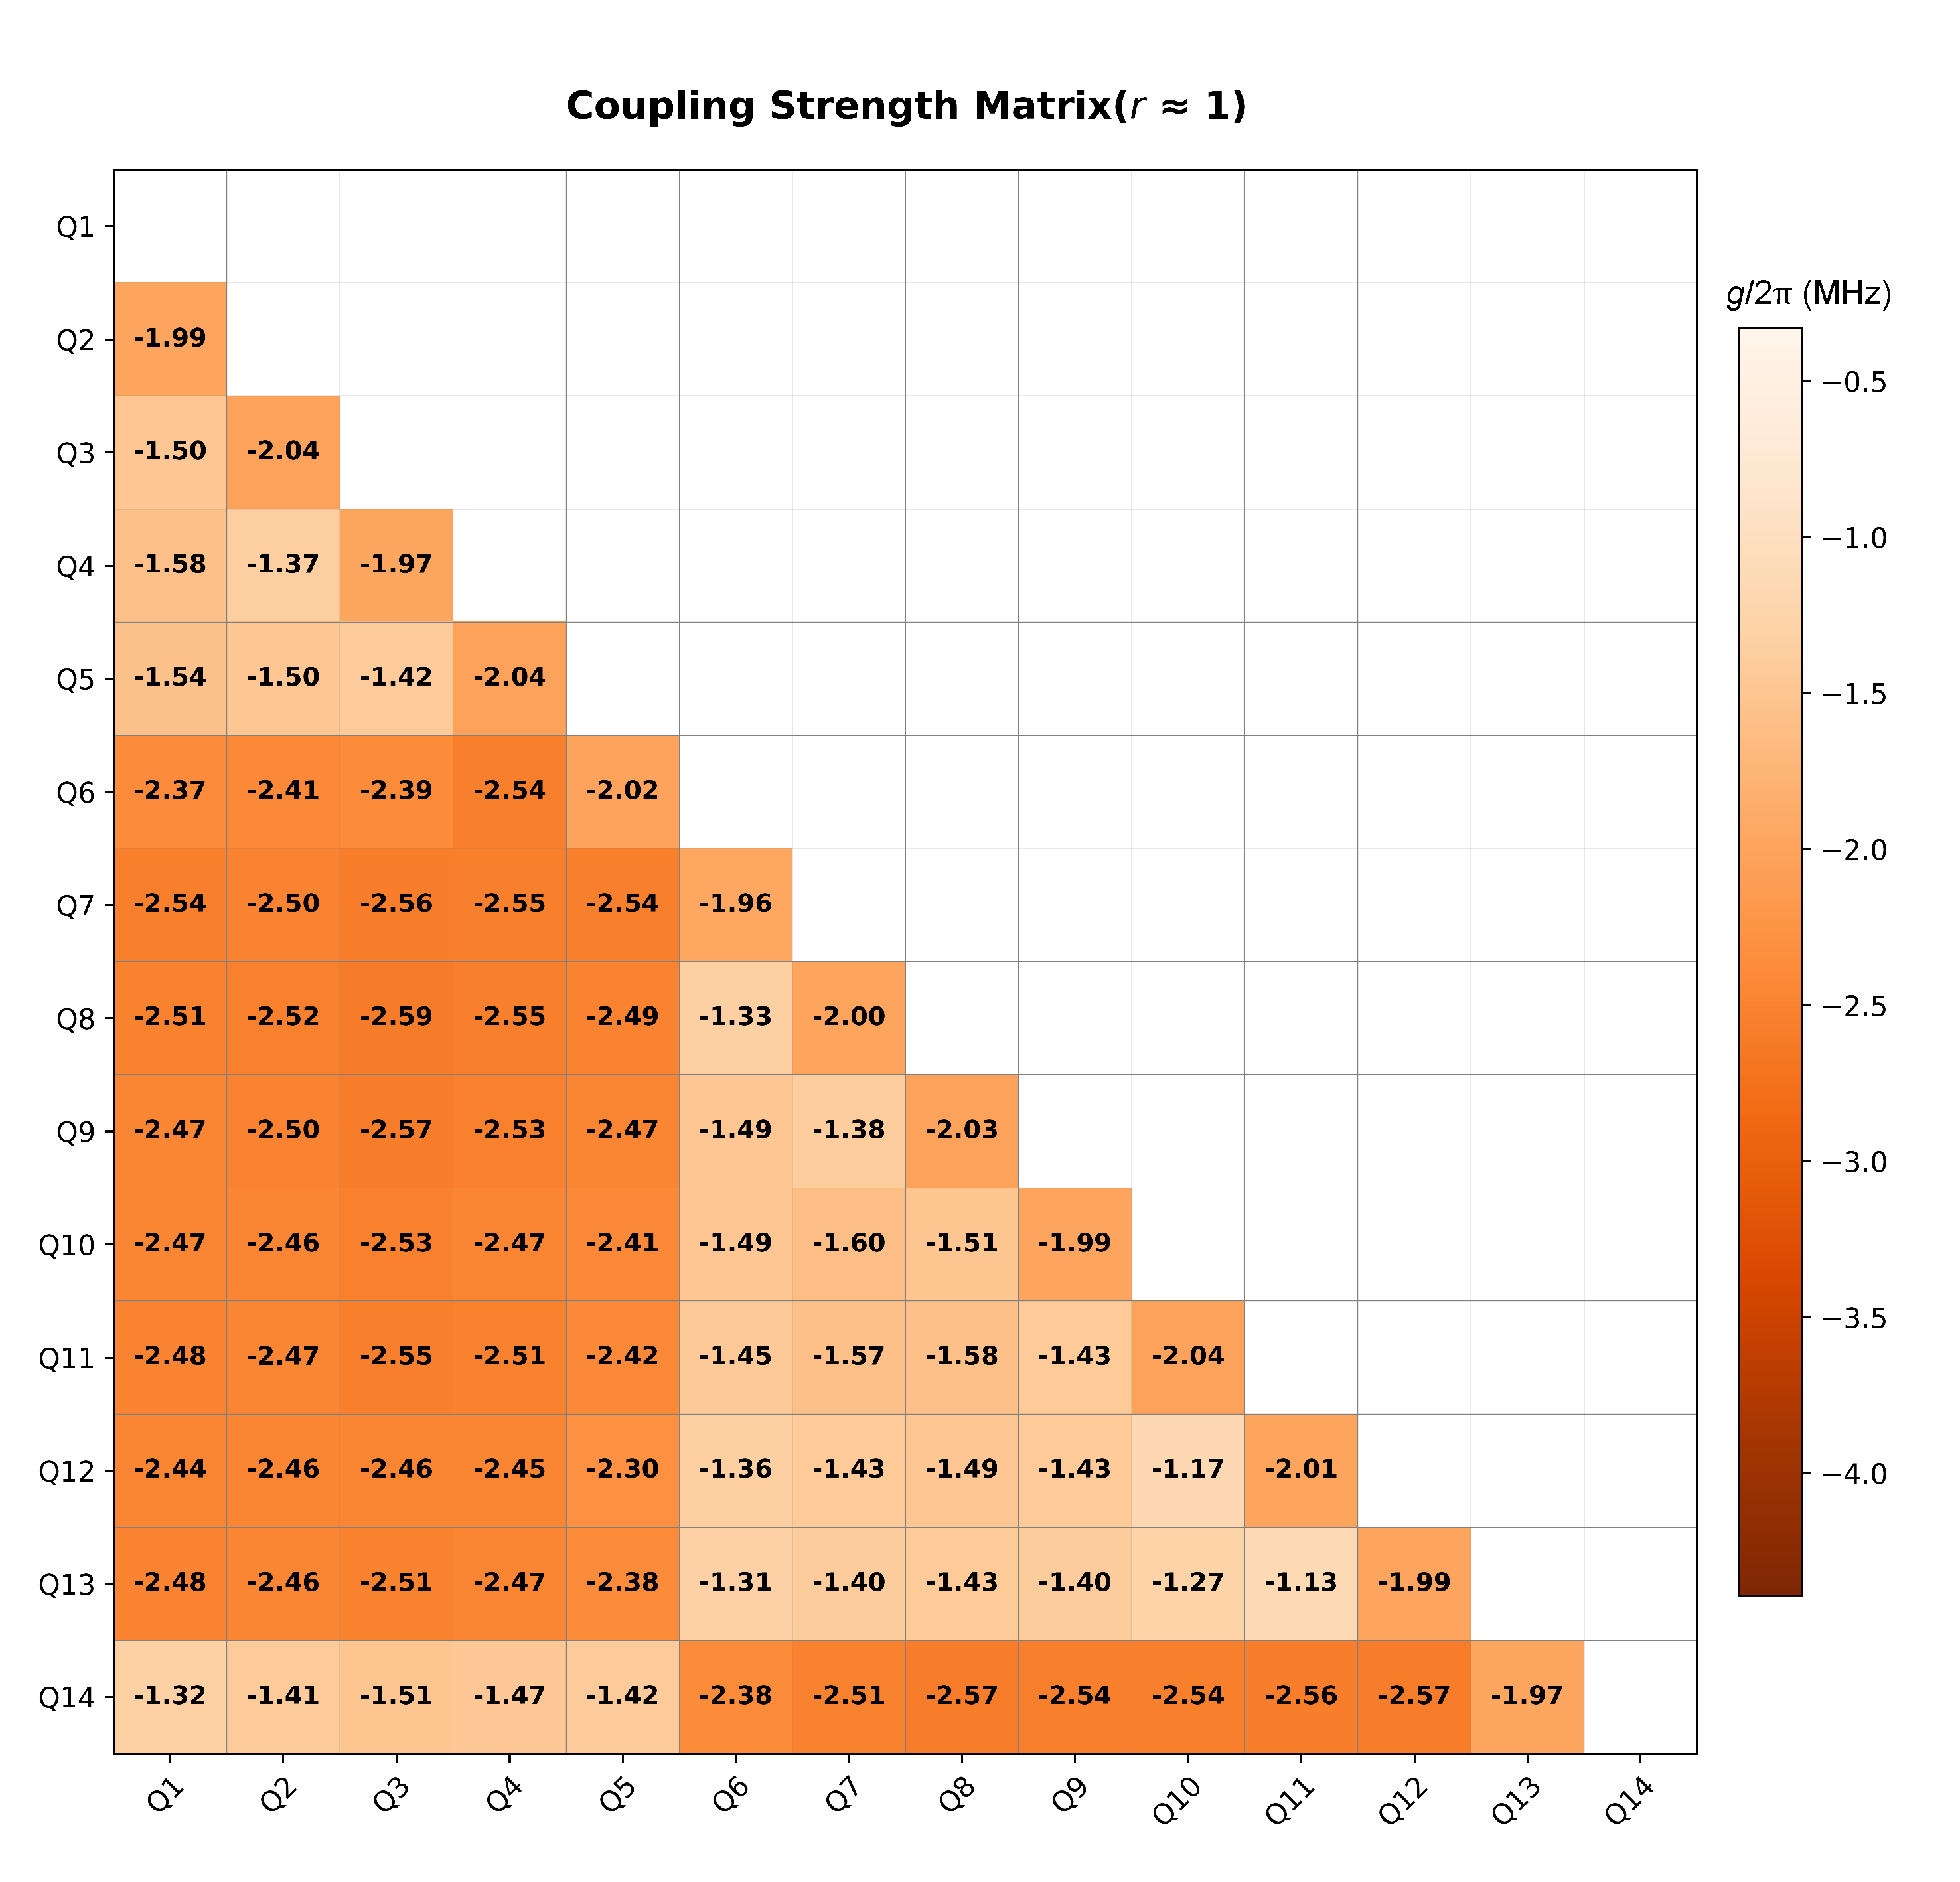
\includegraphics[width=0.7\textwidth]{SupFigS6.pdf}
    \caption{
        \textbf{中间耦合区间($r \approx 1$)的耦合强度矩阵。}
        该图展示了在中间耦合区间下,所有14个量子比特之间的耦合强度分布。
        颜色深浅和线条粗细表示耦合强度$g/2\pi$的大小,单位为MHz。
        在此配置下,最近邻耦合强度设置为$g_N/2\pi = -2$ MHz,长程耦合强度调谐至约$-2$ MHz。
        \textcolor{magenta}{耦合矩阵呈现出较为均匀的分布特征,反映了系统在中间耦合区间的全连接特性,
        此时系统行为由热化过程主导,量子Mpemba效应被抑制。}
    }
    \label{fig:coupling_matrix_intermediate}
\end{figure}

\begin{figure}[H]
    \centering
    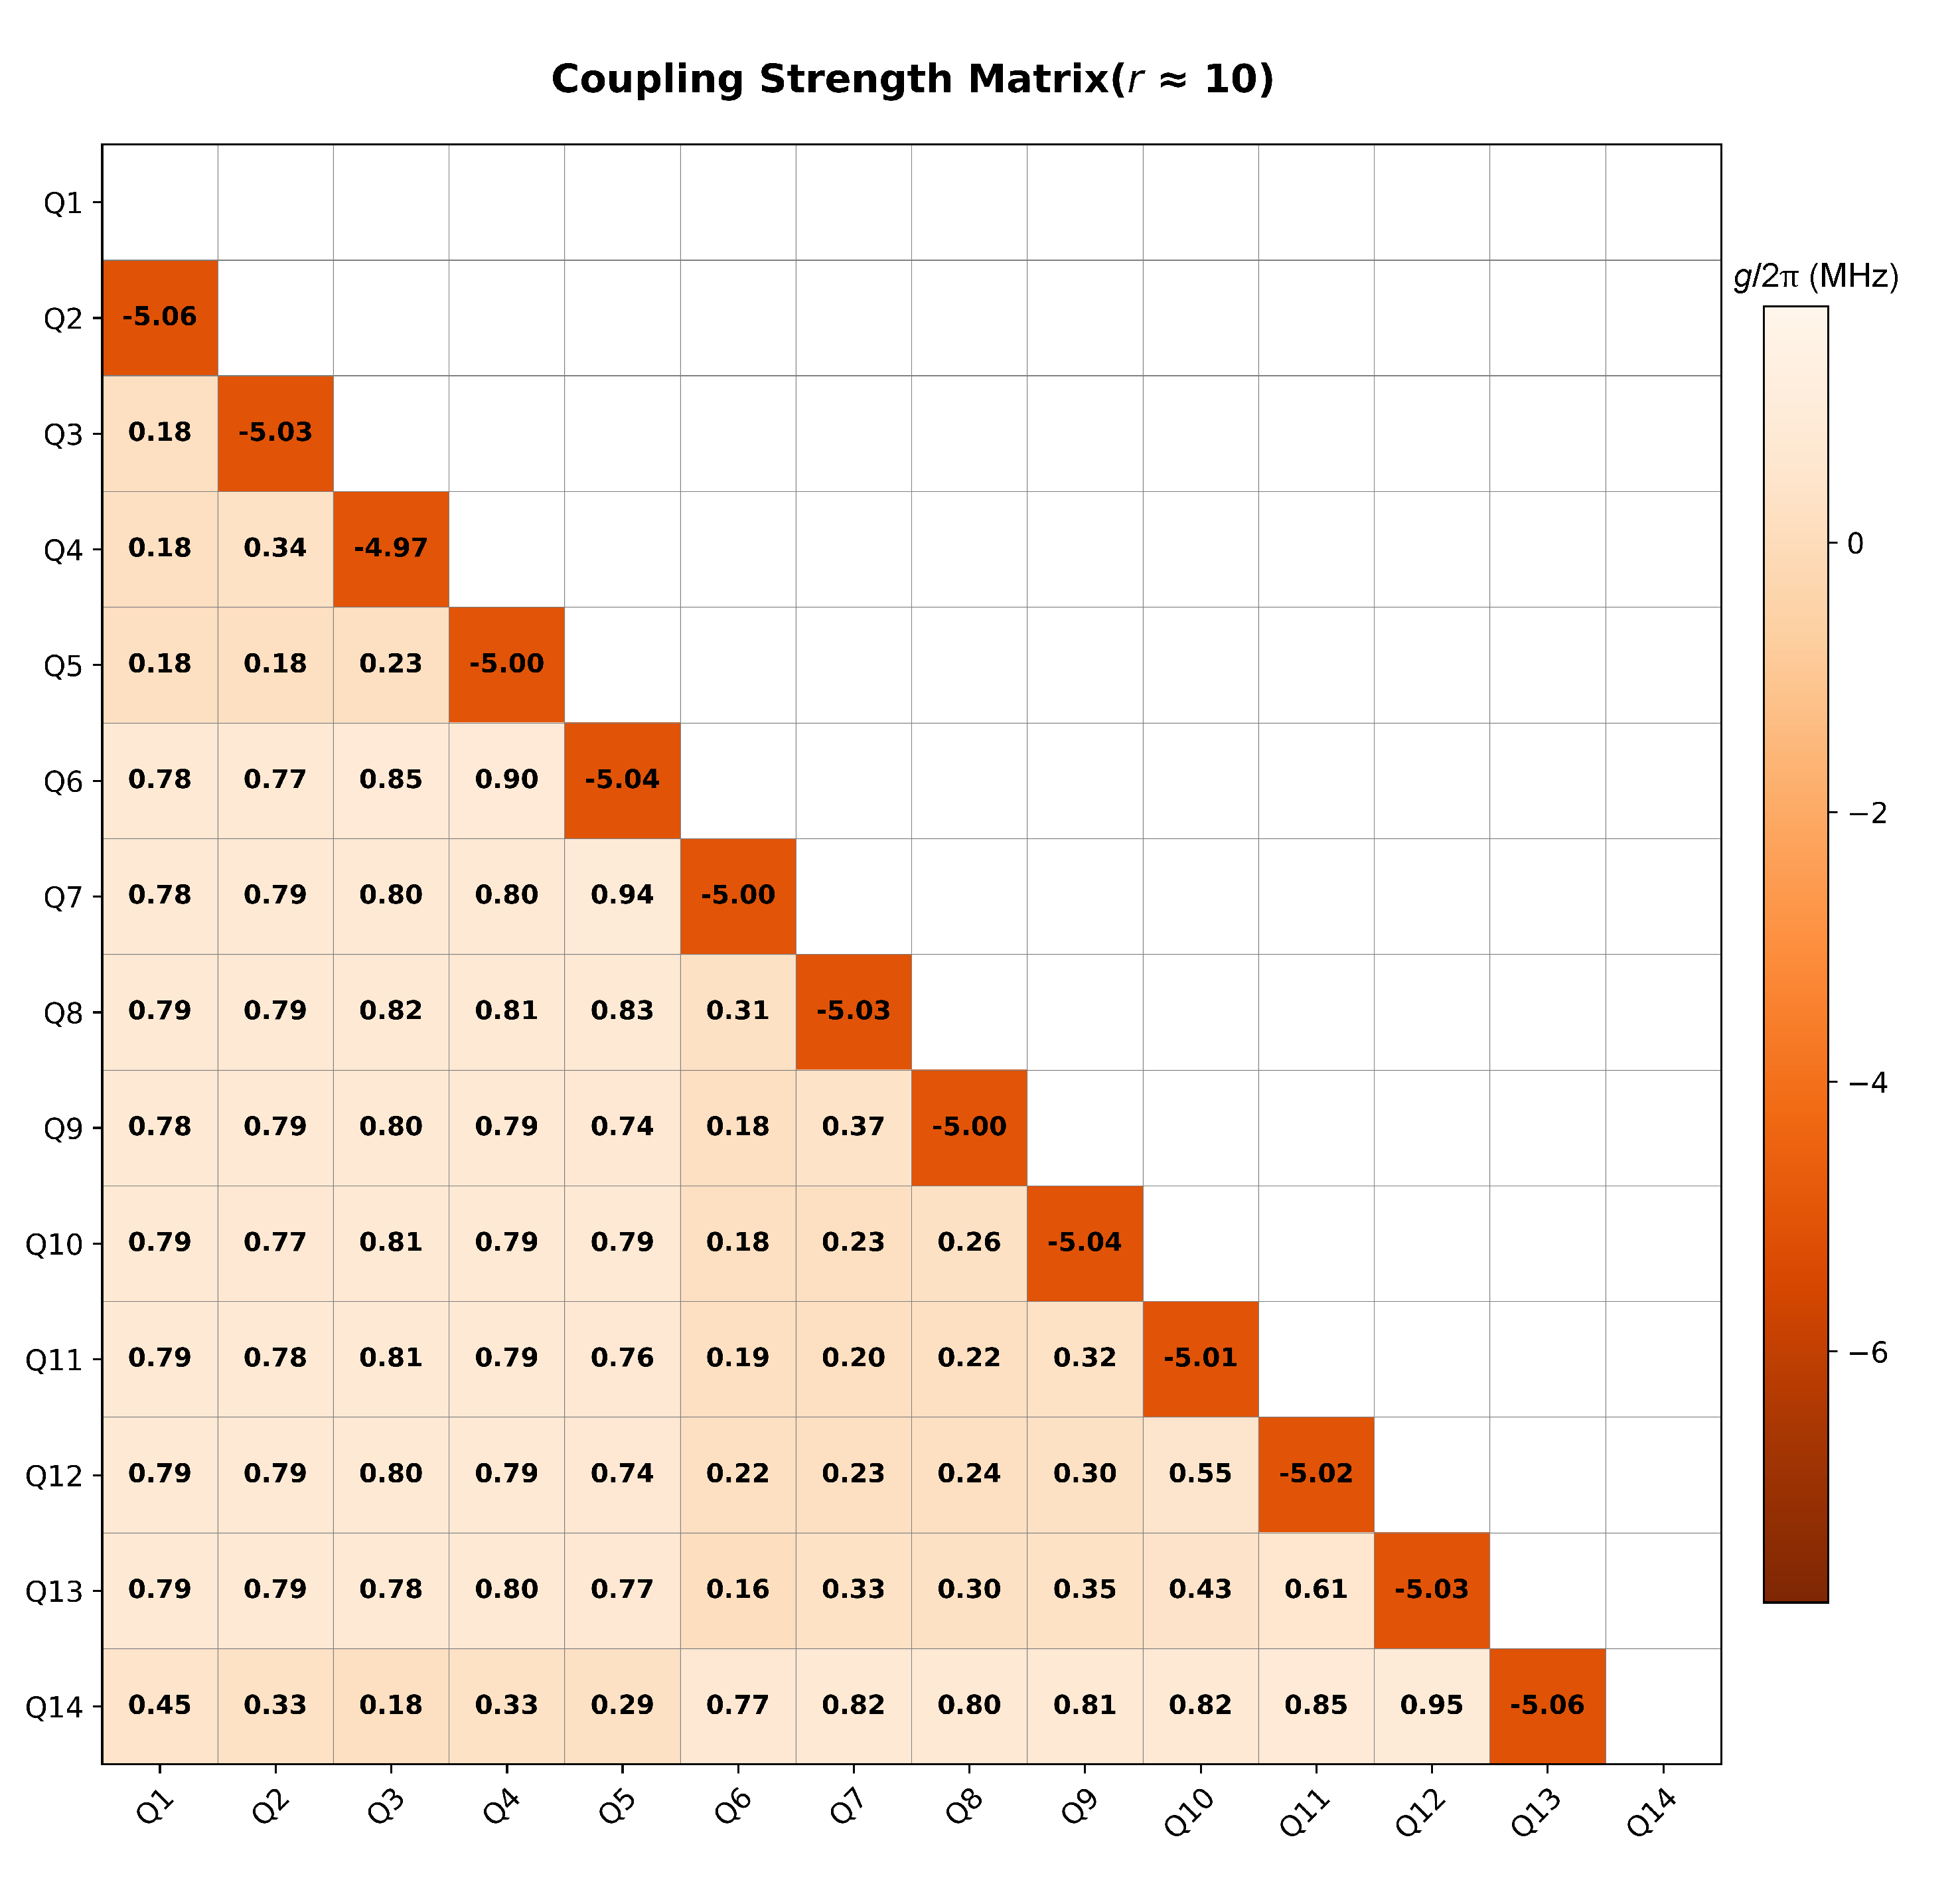
\includegraphics[width=0.7\textwidth]{SupFigS7.pdf}
    \caption{
        \textbf{强短程耦合区间($r \approx 10$)的耦合强度矩阵。}
        该图展示了在强短程耦合区间下,量子比特间的耦合强度分布。
        在此配置中,中心总线谐振器调谐至其最高频率,导致平均长程耦合强度约为$0.5$ MHz,
        而最近邻耦合强度通过耦合器设置为$g_N/2\pi = -5$ MHz。
        \textcolor{magenta}{耦合矩阵显示出明显的最近邻主导特征,长程相互作用被显著抑制,
        此时系统近似映射到可积的一维XX自旋链,为准粒子机制和量子Mpemba效应的出现提供了条件。}
    }
    \label{fig:coupling_matrix_strong_short_range}
\end{figure}



\section{数值模拟}

\subsection{强短程相互作用区间的EA动力学}

我们考虑由方程(2)描述的超导电路理想模型,系统尺寸$N=14$,具有开放边界条件。哈密顿量由下式给出:
\[
H = \sum_{i=1}^{N-1} \left(\sigma_x^i \sigma_x^{i+1} + \sigma_y^i \sigma_y^{i+1}\right) + g \sum_{i+1<j} \left(\sigma_x^i \sigma_x^j + \sigma_y^i \sigma_y^j\right)
\]
其中最近邻相互作用在所有位点均匀,长程相互作用表现出类似的均匀性,$g=1/r$表示长程相互作用的强度。

\begin{figure}[H]
    \centering
    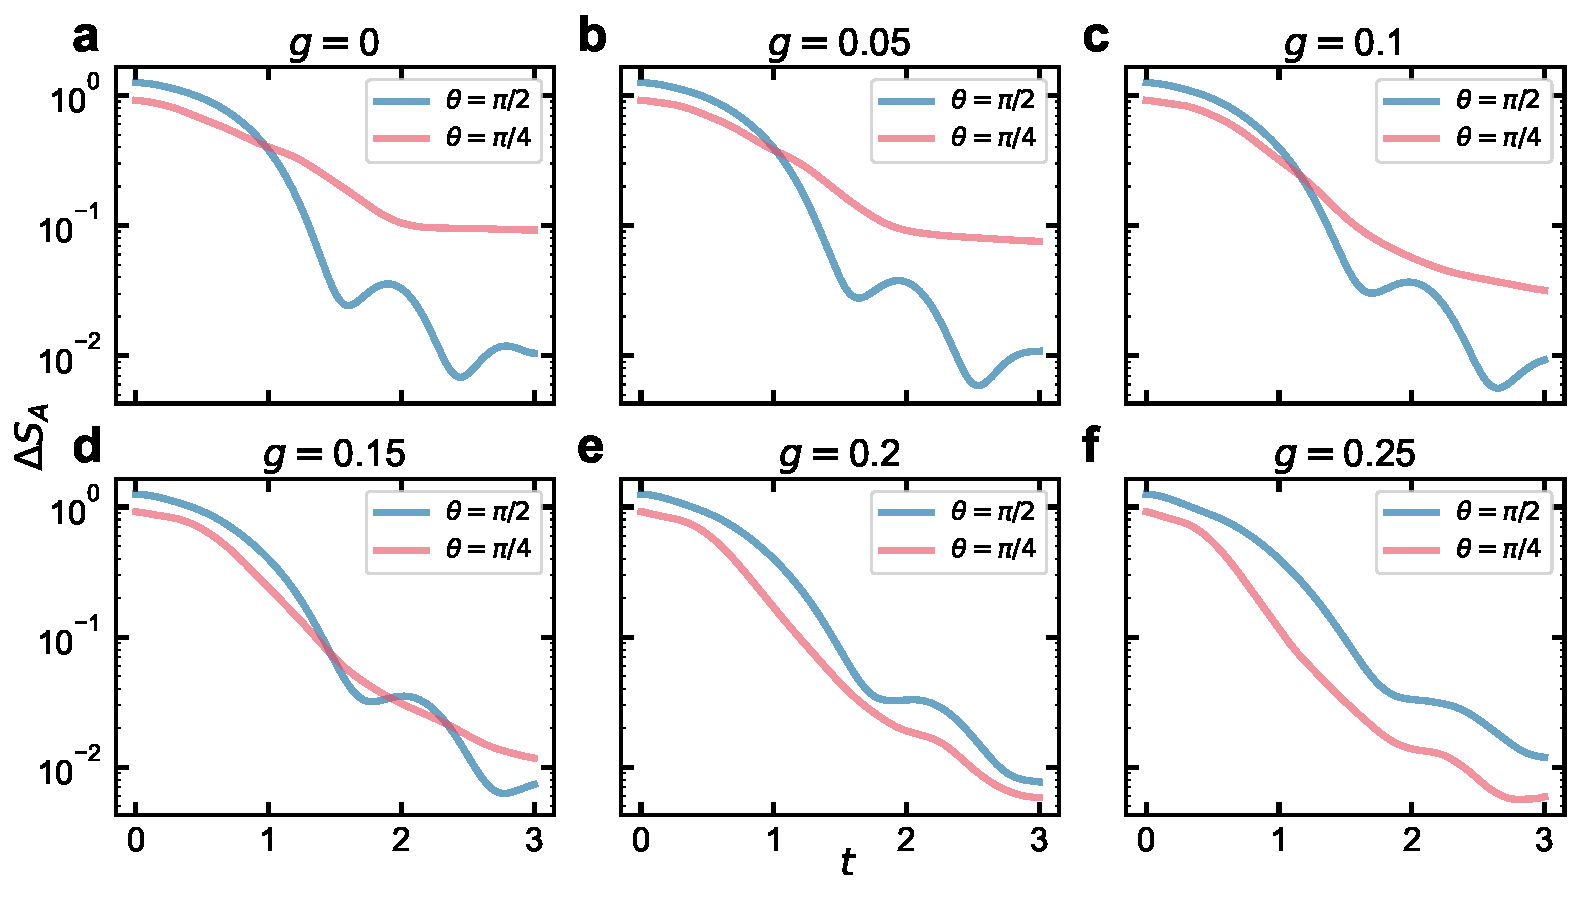
\includegraphics[width=0.9\textwidth]{SupFigS8.pdf}
    \caption{
        \textbf{跨越可积性破缺区间的EA动力学。}
        (a) $g=0$(精确可积极限)时的EA动力学,表现出QME。
        (b-d) 弱可积性破缺区间($g=0.05,0.1,0.15$):早期动力学保留了可积性的特征,包括QME。
        (e-f) 强可积性破缺区间($g=0.2,0.25$):即使在早期时间,热化也占主导,抑制了QME。
        所有模拟都是针对具有开放边界的14自旋链的终端子系统[$Q_1$,$Q_2$,$Q_3$]进行的。
    }
    \label{fig:EA_dynamics_integrability}
\end{figure}

在可积极限($g=0$)下,哈密顿量简化为XX自旋链,通过Jordan-Wigner变换可精确求解为自由费米子。对此类可积模型中EA的理论研究揭示,QME允许准粒子解释:子系统内产生的纠缠准粒子对贡献于EA,而在外部传播的准粒子则不贡献。关键见解是,更不对称的初始态激发传播更快的模式,加速EA衰减。这一准粒子框架解释了观察到的有限尺寸振荡和边界效应。

对于弱可积性破缺,哈密顿量包含引入有限准粒子寿命的扰动。尽管如此,早期动力学仍然与可积模型预测一致。相反,当相互作用比超过某一阈值时,热化主导动力学,导致基本不同的行为,表现为QME特征的消失。

\subsection{倾斜铁磁态在$r=1$时的解析结果}

当相互作用比$r=1$时,系统动力学在集体自旋图像中允许精确解析解。对于$N$个自旋-1/2量子比特系统,集体自旋算符定义为:
\[
\bm{S} = \frac{1}{2} \sum_{i=1}^{N} \bm{\sigma}^i
\]

全连接的XX相互作用哈密顿量变换为:
\[
H = g\left(S_x^2 + S_y^2 - \frac{N}{2}\right) = g\left(\bm{S}^2 - S_z^2 - \frac{N}{2}\right)
\]
其中常数项$-N/2$仅贡献全局相位,因此可忽略。希尔伯特空间分解为角动量扇区,基态为$|S,m\rangle$,其中$S$表示总自旋量子数(对于偶/奇$N$,范围从$0$或$1/2$到$N/2$),$m$表示磁量子数($m=-S,\ldots,S$)。最大自旋扇区$S=N/2$精确对应于Fock空间,基态通过下式映射到计算基态:
\[
|S=\frac{N}{2}, m=\frac{N}{2}-n\rangle = \frac{1}{\sqrt{\binom{N}{n}}}(\sigma^{-})^n |0\rangle^{\otimes N}
\]
其中$\binom{N}{n}$是二项式系数,$\sigma^{-}=\sum_{i=1}^{N}\sigma_i^{-}$是集体降低算符,$|0\rangle^{\otimes N}$是全自旋向上态,$n$索引激发量子比特的数量($n=0,1,\ldots,N$)。

倾斜铁磁初始态可以在以下表示中表达:
\[
|\theta\rangle_F = \left(\cos\frac{\theta}{2}|0\rangle + \sin\frac{\theta}{2}|1\rangle\right)^{\otimes N}
= \sum_{n=0}^{N} \left(\cos\frac{\theta}{2}\right)^{N-n} \left(\sin\frac{\theta}{2}\right)^n \sqrt{\binom{N}{n}} |S=\frac{N}{2}, m=\frac{N}{2}-n\rangle
\]

这种相干叠加跨越所有激发扇区$n$。在从$|\theta\rangle_F$淬火的动力学下,$\bm{S}^2$成为守恒量,将有效哈密顿量简化为Lipkin-Meshkov-Glick (LMG)模型:
\[
H_{\text{eff}} = -gS_z^2
\]

哈密顿量的对角结构产生精确的时间演化:
\[
|\Psi(t)\rangle = e^{-iH_{\text{eff}}t}|\theta\rangle_F = \sum_{n=0}^{N} \left(\cos\frac{\theta}{2}\right)^{N-n} \left(\sin\frac{\theta}{2}\right)^n \sqrt{\binom{N}{n}} e^{igt(N/2-n)^2} |S=\frac{N}{2}, m=\frac{N}{2}-n\rangle
\]

周期性复兴$|\Psi(t=T_S)\rangle \propto |\Psi(0)\rangle$以复兴周期出现:
\[
T_S = \begin{cases}
2\pi/g & \text{偶 } N \\
\pi/g & \text{奇 } N
\end{cases}
\]

对于EA分析,我们将总自旋$\bm{S} = \bm{S}^A + \bm{S}^{\overline{A}}$划分为子系统$A$($N_A$个量子比特)及其补集$\overline{A}$,对于实验相关性取偶$N$。哈密顿量变为:
\[
H_{\text{eff}} = -g\left[(S_z^A)^2 + (S_z^{\overline{A}})^2 + 2S_z^A S_z^{\overline{A}}\right]
\]

在最大自旋基$|S_A=N_A/2,m_1\rangle \otimes |S_{\overline{A}}=(N-N_A)/2,m_2\rangle$中工作,其中$m_1$范围从$-N_A/2$到$N_A/2$,$m_2$范围从$-(N-N_A)/2$到$(N-N_A)/2$,子系统$A$保持局限于其$S_A=N_A/2$扇区。结果,$\rho_{A,Q}$是时间无关的,建立:
\[
\Delta S_A(t) = C(\theta) - S_A(\theta,t)
\]
其中$C(\theta)$是依赖于初始态的常数,
\[
C(\theta) = -\ln\sum_{n=0}^{N_A} \cos\left(\frac{\theta}{2}\right)^{4(N_A-n)} \sin\left(\frac{\theta}{2}\right)^{4n} \binom{N_A}{n}^2
\]

\textcolor{magenta}{$C(\theta)$显示出关于$\theta=\pi/2$的完美对称性:它在区间$(0,\pi/2)$内单调增加,在$\theta=\pi/2$处达到最大值,并在$(\pi/2,\pi)$内单调减少。}时间演化态为:
\[
|\Psi(t)\rangle = \sum_{m_1,m_2} C^{N_A}_{m_1}(\theta) C^{N-N_A}_{m_2}(\theta) e^{igt(m_1+m_2)^2} |m_1\rangle \otimes |m_2\rangle
\]
其中系数:
\[
C^{N}_{m}(\theta) = \left(\cos\frac{\theta}{2}\right)^{N/2+m} \left(\sin\frac{\theta}{2}\right)^{N/2-m} \sqrt{\binom{N}{N/2-m}}
\]
其中$|m_1\rangle \equiv |S_A=N_A/2,m_1\rangle$,$|m_2\rangle \equiv |S_{\overline{A}}=(N-N_A)/2,m_2\rangle$。

子系统$A$的约化密度矩阵元素为:
\[
\rho^{A}_{m_1,m^{\prime}_1} = C^{N_A}_{m_1}(\theta) C^{N_A}_{m^{\prime}_1}(\theta) e^{igt(m_1^2-m^{\prime 2}_1)} \sum_{m_2} |C^{N-N_A}_{m_2}(\theta)|^2 e^{2igtm_2(m_1-m^{\prime}_1)}
\]

Renyi-2 EA为:
\[
\Delta S_A = \ln\left(\frac{\operatorname{Tr}(\rho^2_A)}{\operatorname{Tr}(\rho^2_{A,Q})}\right)
= \ln\left(1 + \frac{\sum_{i\neq j}|\rho^A_{i,j}|^2}{\sum_{i}|\rho^A_{i,i}|^2}\right)
= \ln\left(1 + \frac{2\sum_{m_1<m^{\prime}_1}|C^{N_A}_{m_1}(\theta)C^{N_A}_{m^{\prime}_1}(\theta)|^2 \mathcal{C}(m_1,m^{\prime}_1)}{\sum_{m_1}|C^{N_A}_{m_1}(\theta)|^4 \left(\sum_{m_2}|C^{N-N_A}_{m_2}(\theta)|^2\right)^2}\right)
\]
其中因子$\mathcal{C}(m_1,m^{\prime}_1) = \sum_{m_2,m^{\prime}_2}|C^{N-N_A}_{m_2}(\theta)C^{N-N_A}_{m^{\prime}_2}(\theta)|^2 \cos[2gt(m_1-m^{\prime}_1)(m_2-m^{\prime}_2)]$捕获了子系统的内部相干性。

由于$(m_1-m^{\prime}_1)$和$(m_2-m^{\prime}_2)$是整数,EA以周期$T_{\text{EA}} = \pi/g$振荡。在$t=T_{\text{EA}}$时:
\[
|\Psi(t)\rangle \propto |-\theta\rangle_F
\]
由于$|-\theta\rangle_F = e^{-i\pi S_z}|\theta\rangle_F$,EA与$|\theta\rangle_F$相同。

\begin{figure}[H]
    \centering
    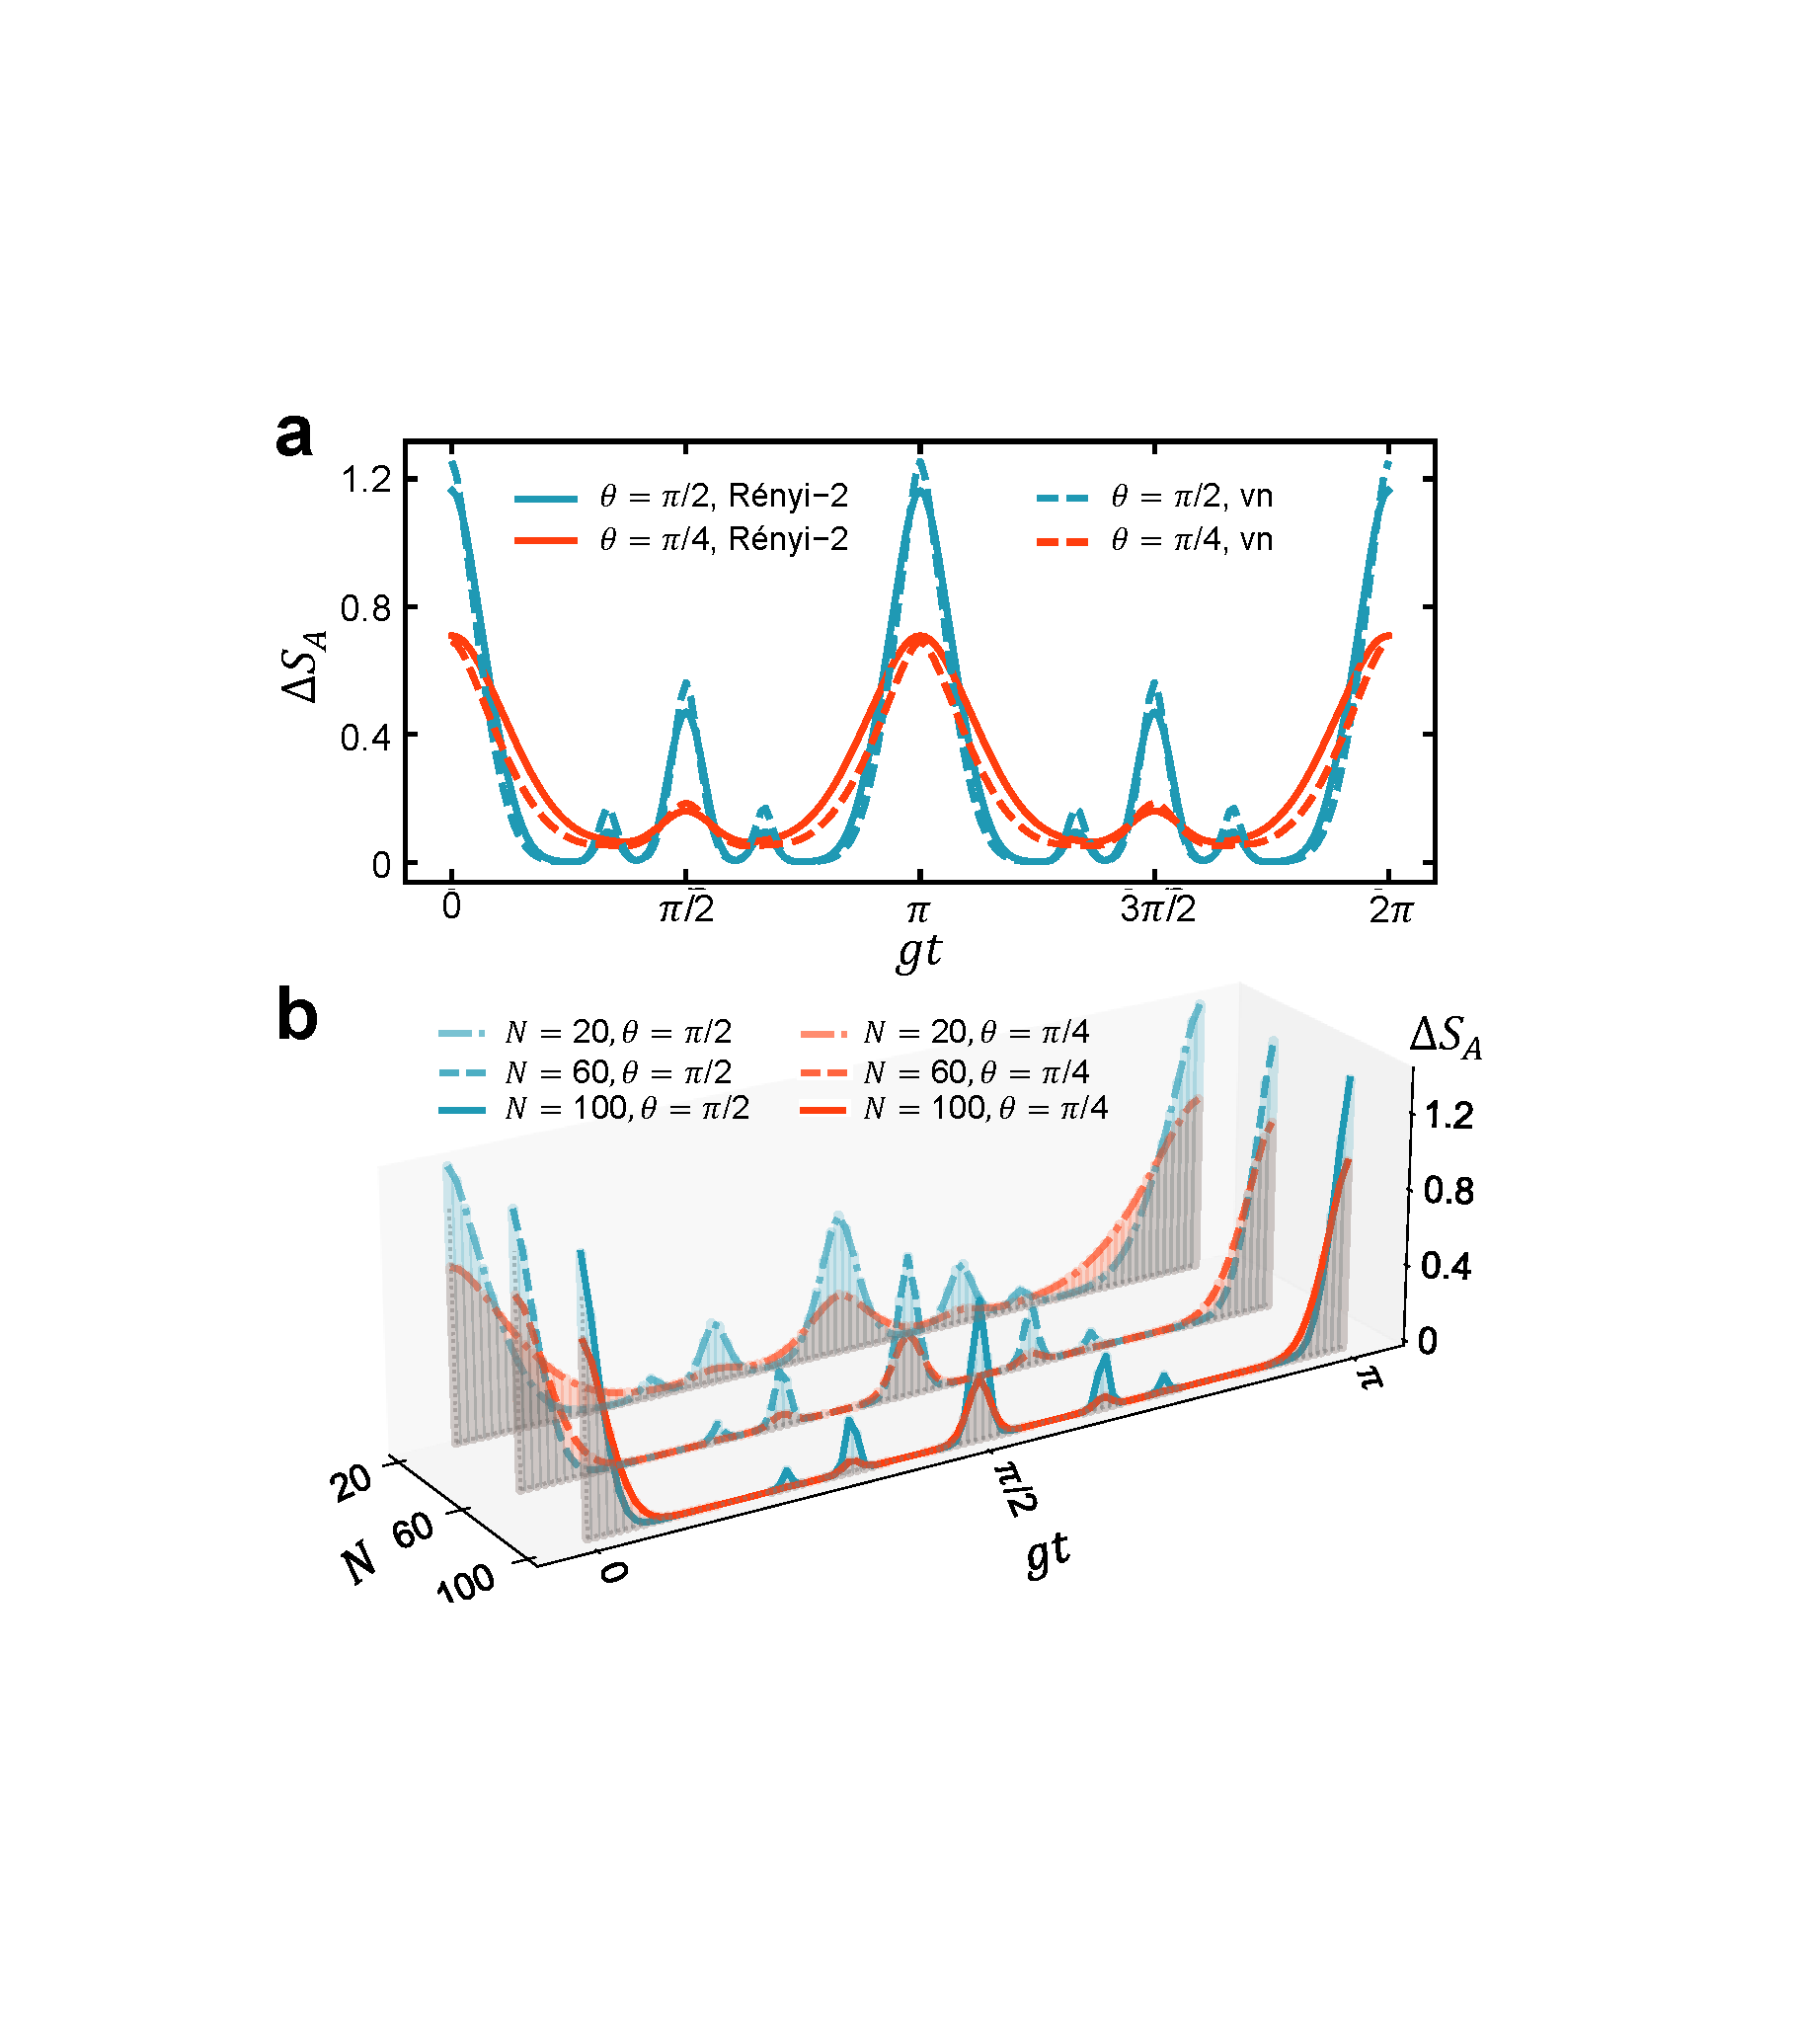
\includegraphics[width=0.7\textwidth]{SupFigS9.pdf}
    \caption{
    \textbf{Supplementary Fig. S9. 不同度量与系统尺寸下的 EEA 动力学。}
    \textbf{a,} 在 $N = 14$ 的自旋链中,子系尺寸 $N_a = 3$ 时分别使用冯·诺依曼熵和 Rényi-2 熵计算的 EA 动力学对比。尽管绝对值略有差异,两种度量捕捉到的动力学特征完全一致。
    \textbf{b,} 固定 $N_a = 4$ 时 EA 动力学(冯·诺依曼熵)的系统尺寸依赖性。随着 $N$ 增大,子系对称性恢复加速并趋于完全,而特征动力学交叉行为保持不变。
    }
    \label{fig:S9}
\end{figure}

\begin{figure}[H]
    \centering
    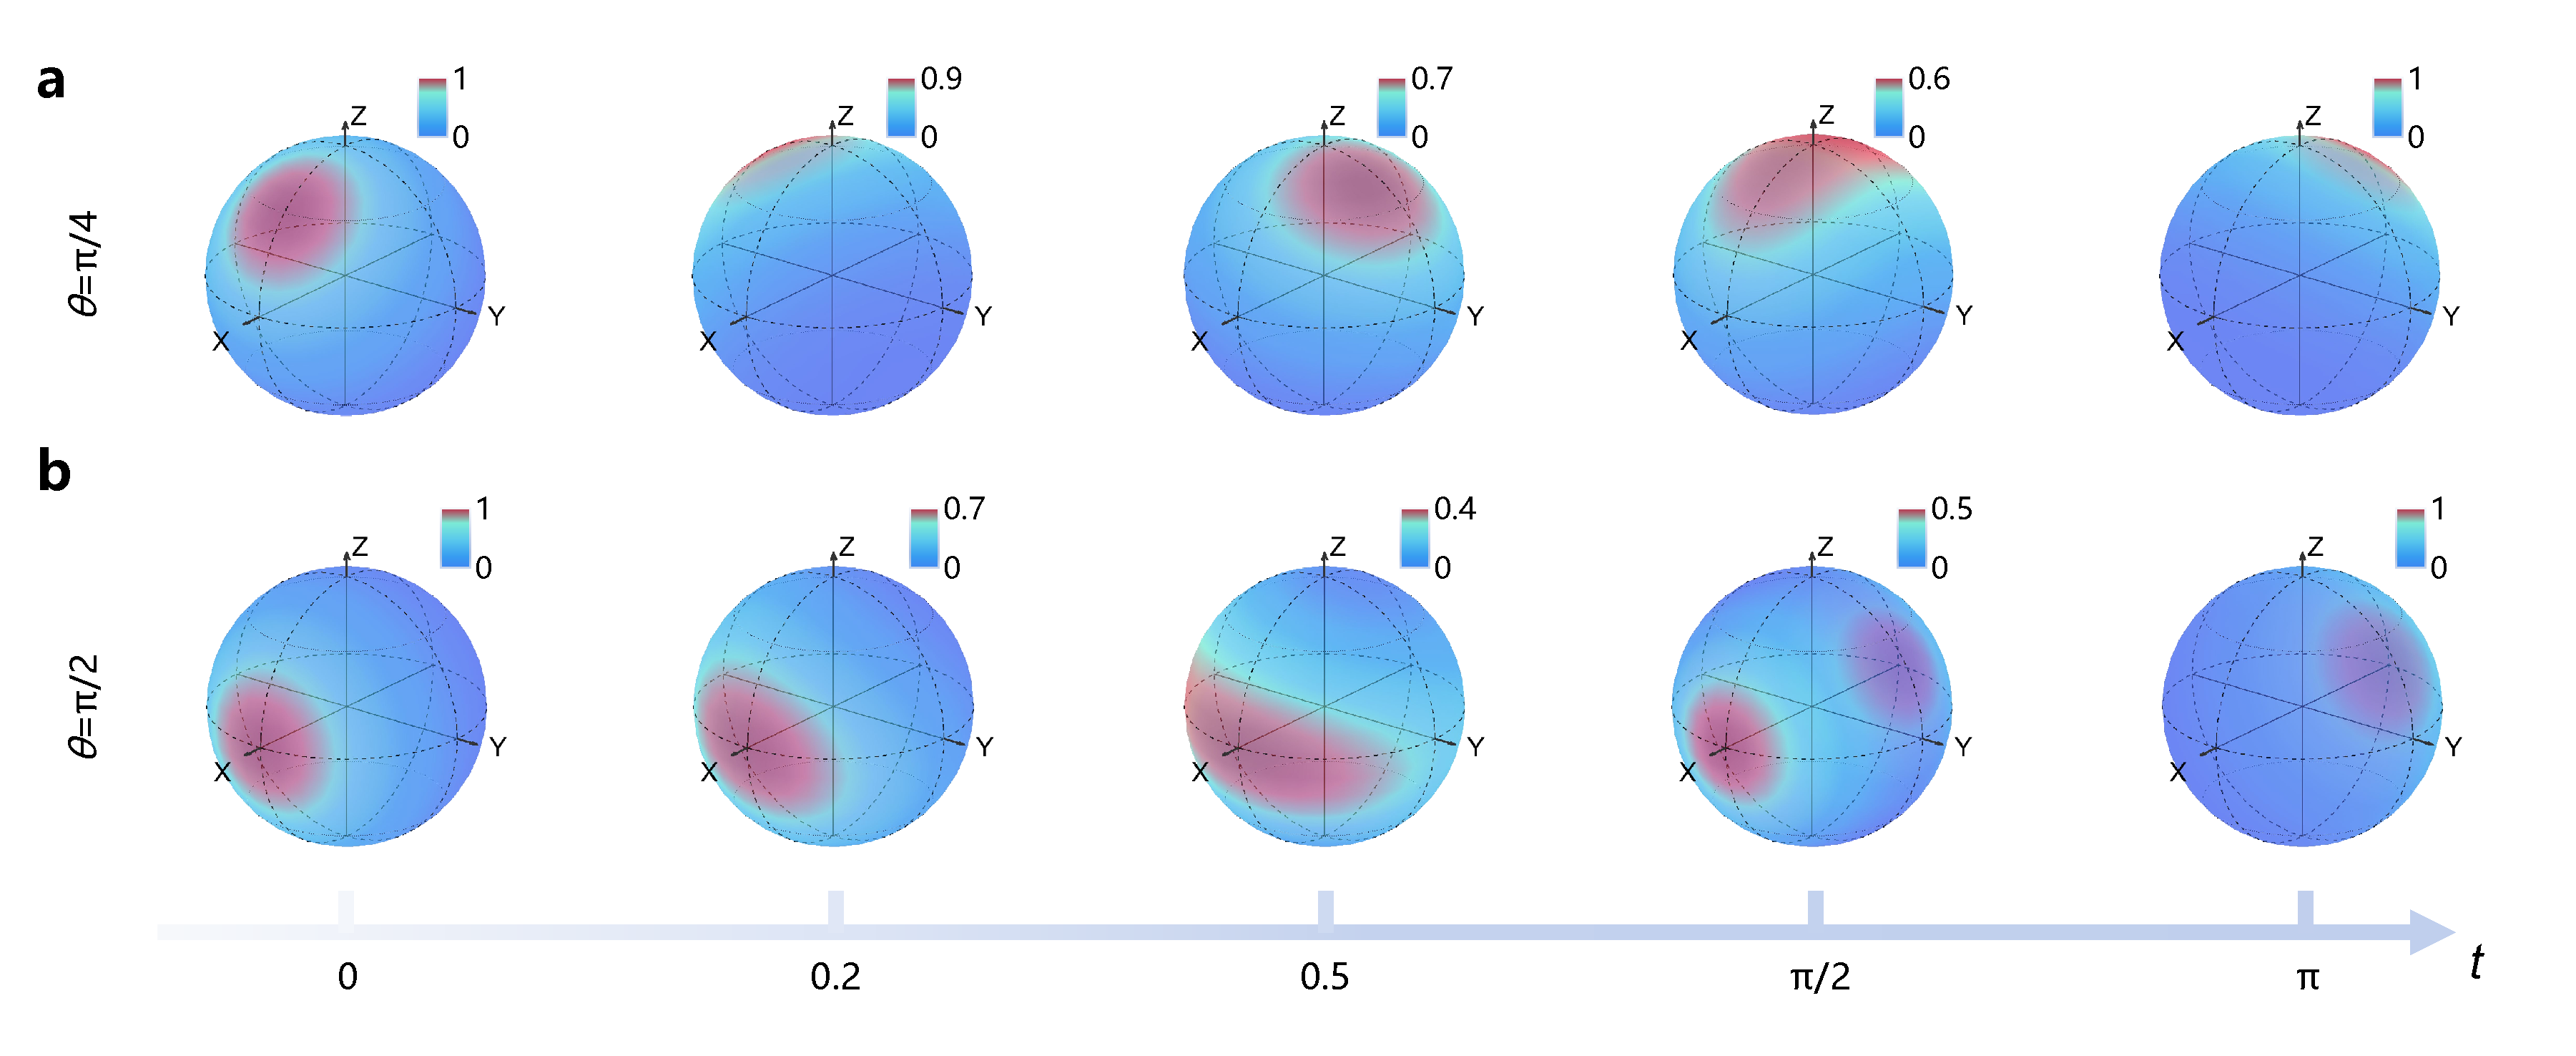
\includegraphics[width=0.95\textwidth]{SupFigS10.pdf}
    \caption{
        \textbf{准分布函数的动力学。}
        (a) $\theta=\pi/4$和(b) $\theta=\pi/2$的演化。
        方位角分布向均匀性演化,反映了$U(1)$对称性的恢复。
        值得注意的是,与$\pi/4$相比,$\theta=\pi/2$处的更快平坦化展示了QME。
        关键特征包括:(i) 在$t=T_{\text{EA}}/2$处的$Z_2$对称分岔(部分$U(1)$恢复),和(ii) 在EA周期的两倍($T_S=2T_{\text{EA}}$)处的完全复兴,因为分布返回到与初始态对称的配置。
        系统尺寸$N=14$和$N_A=3$,与实验设置匹配。
    }
    \label{fig:quasidistribution_dynamics}
\end{figure}

为了可视化对称性恢复动力学,我们使用准分布函数$Q(\theta,\phi)=\langle\theta,\phi|\rho_A|\theta,\phi\rangle$,其中\textcolor{magenta}{相干自旋态}定义为$|\theta,\phi\rangle=e^{-i\phi\sum_i\sigma_z^{(i)}/2}e^{-i\theta\sum_i\sigma_y^{(i)}/2}|00\cdots 0\rangle$。最初($t=0$),分布沿着特定方向尖锐峰值。随着系统演化,方位角($\phi$方向)分布逐渐变得均匀,标志着$U(1)$旋转对称性的恢复。与$\theta=\pi/4$相比,$\theta=\pi/2$的分布更快平坦化直接体现了QME。在$t=T_{\text{EA}}/2$时,分布分岔为两个对称峰,揭示了涌现的$Z_2$对称性和部分$U(1)$对称性恢复。到$t=T_{\text{EA}}$时,分布复兴到与初始态对称的配置,展示了关系$T_S=2T_{\text{EA}}$。至关重要的是,这些$Q(\theta,\phi)$动力学提供了在可积LMG模型中对称性恢复的完整可视化——这个过程不能通过传统的准粒子传播来解释。

\subsection{在位势对EA动力学的影响}




我们的工作进一步研究了在位势与QME之间的关系,检查了线性势对倾斜Néel态的影响以及无序对$r\approx 1$区间中倾斜铁磁态的影响。

在没有在位势的情况下,对于倾斜Néel态,较小倾斜角的对称性恢复更快,从而抑制QME。这一行为得到了纠缠动力学测量的证实,其中纠缠熵线性增加然后饱和。鉴于倾斜Néel态的小能量差(对于$\theta=\pi/4$,$\langle H\rangle/(e_{\text{max}}-e_{\text{min}})=0.03$,而对于$\theta=\pi/2$,为$0.06$,其中$e_{\text{max}}$和$e_{\text{min}}$分别表示系统的最大和最小本征能量),两种状态自然演化到相同的稳态,它们的EE在Page值处饱和。\textcolor{magenta}{在这种情况下,EE作为热化速率的指标。EE的时间演化紧密反映了EA动力学,证实了热化更快的状态更快地恢复对称性。这种相关性源于热化驱动系统朝向$U(1)$对称的热吉布斯系综,本质上将热化与对称性恢复联系起来。}

\begin{figure}[H]
    \centering
    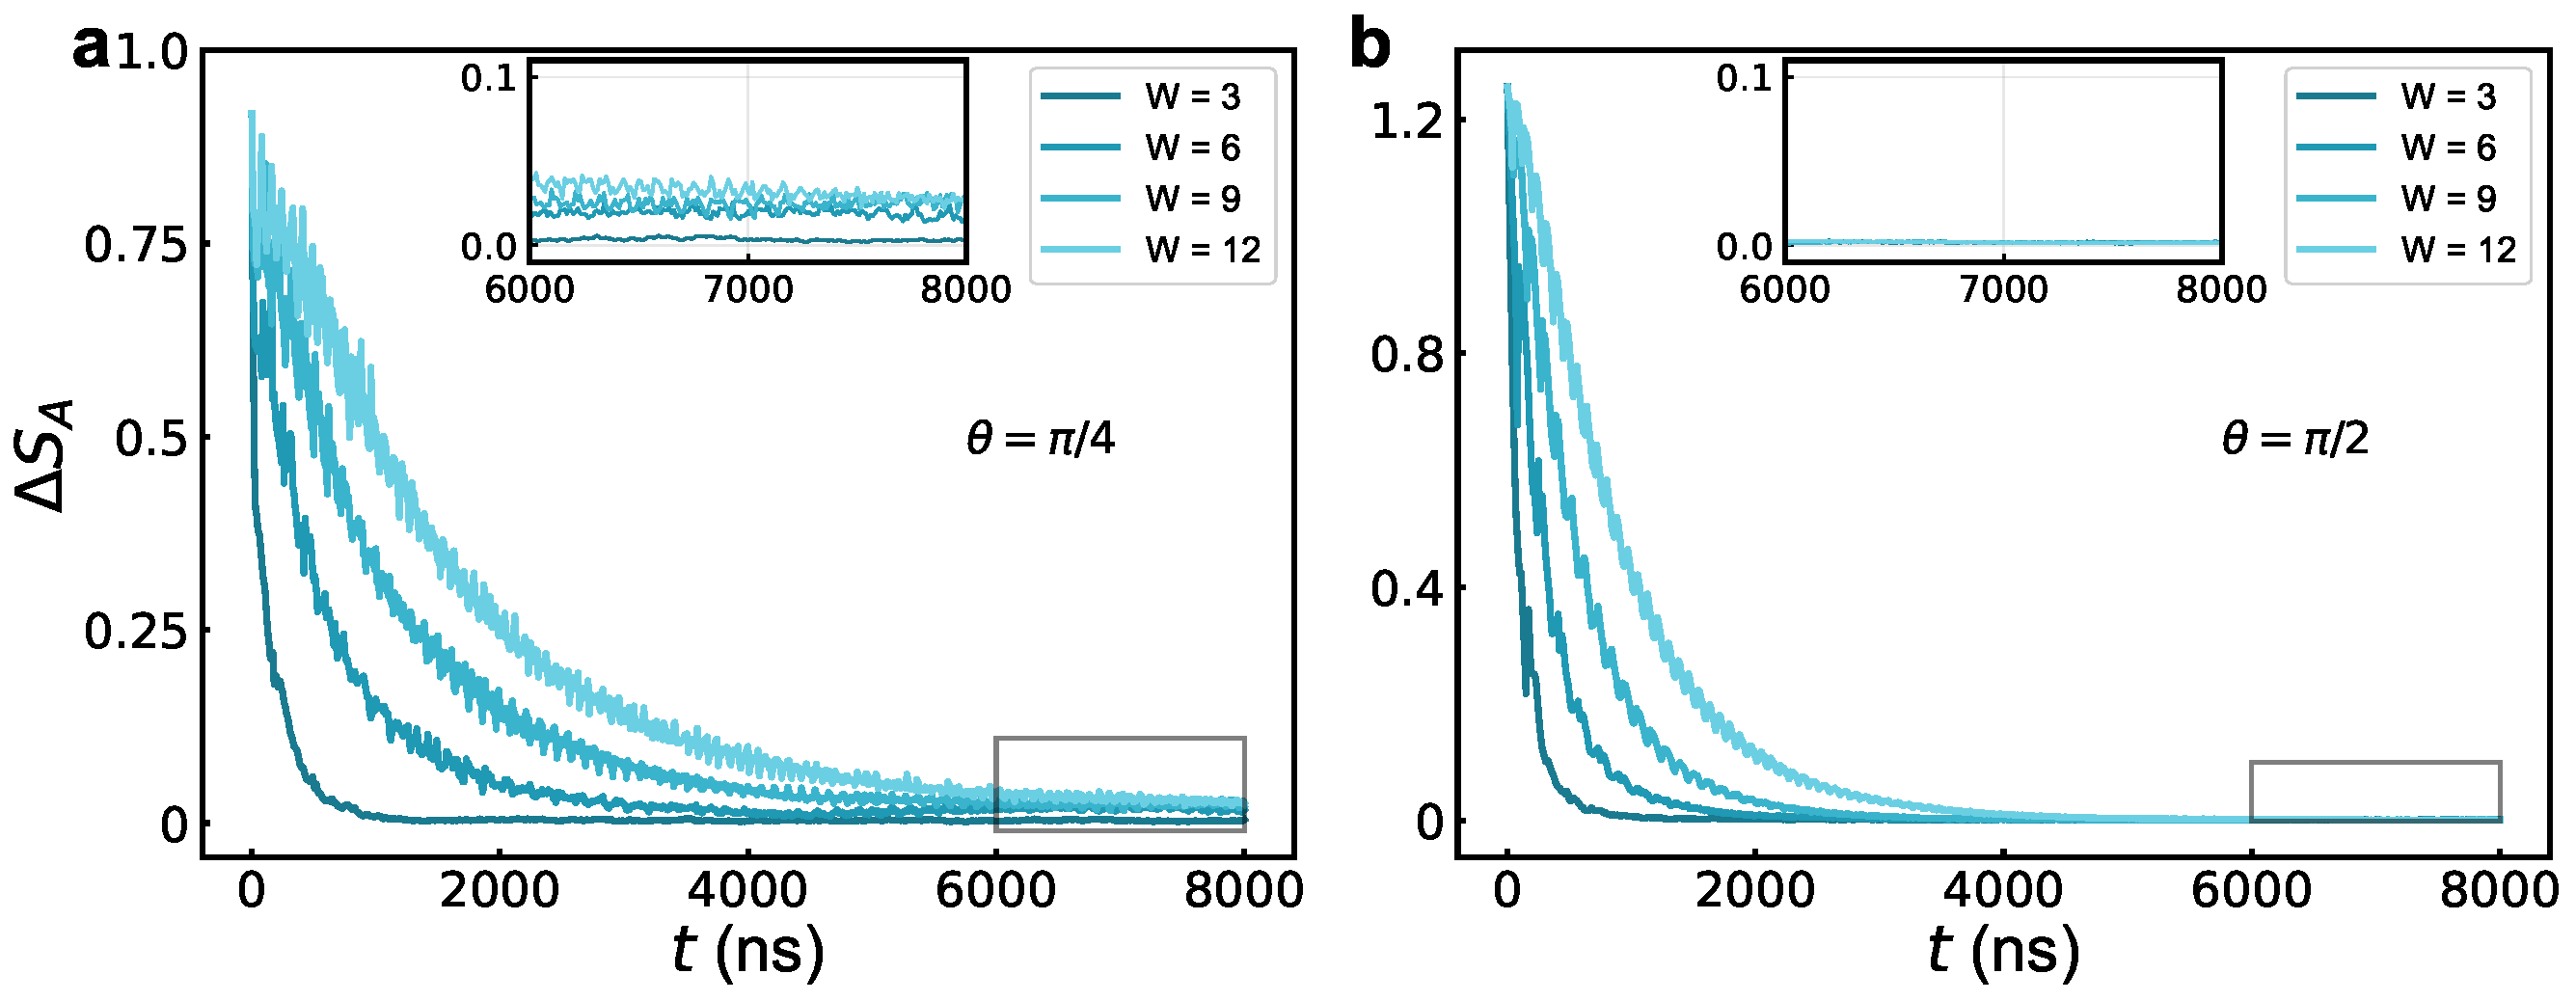
\includegraphics[width=0.95\textwidth]{SupFigS11.pdf}
    \caption{
        \textbf{在位势对纠缠不对称性长期行为的影响。}
        该图展示了在不同线性势强度$W$下,倾斜Néel态的纠缠不对称性(EA)长期演化行为。
        (a) 随着线性势强度$W$的增加,倾斜角$\theta=\pi/4$的EA长期值逐渐上升,表明对称性恢复过程受到抑制。
        (b) 相比之下,倾斜角$\theta=\pi/2$的EA长期值几乎保持不变,显示出对线性势的较弱敏感性。
        这种角度依赖的响应导致了EA曲线的交叉现象,使得量子Mpemba效应在中间耦合区间重新出现。
        结果验证了通过引入线性势可以调控对称性恢复速率,为量子动力学的可控调制提供了实验依据。
    }
    \label{fig:onsite_potential_EA_effects}
\end{figure}

在强线性势下,尽管对称性恢复整体减慢,但抑制程度取决于倾斜角$\theta$——具有较大$\theta$的状态显示较弱的抑制,因此QME恢复。如图所示,跨势强度$W$的长时间行为的数值模拟揭示,对于$\theta=\pi/2$,$\Delta S_A(t\rightarrow\infty)$几乎保持不变,但对于$\theta=\pi/4$,在研究范围内增加,满足:
\[
\Delta S_A(\pi/4,t=0) < \Delta S_A(\pi/2,t=0)
\]
\[
\Delta S_A(\pi/4,t\rightarrow\infty) > \Delta S_A(\pi/2,t\rightarrow\infty)
\]

我们将这种现象归因于势诱导的遍历性破缺。支持证据来自两个关键观察:(i) 平均能级间距比接近泊松极限($\langle r\rangle \rightarrow 0.386$),计算为:
\[
\langle r\rangle = \frac{1}{N}\sum_{n=1}^{N} \frac{\min(\delta_n,\delta_{n+1})}{\max(\delta_n,\delta_{n+1})}
\]
其中$\delta_n=E_n-E_{n-1}$表示相邻本征能量间隙。(ii) 随着势强度$W$增加,不平衡表现出持续的非零值。

\begin{figure}[H]
    \centering
    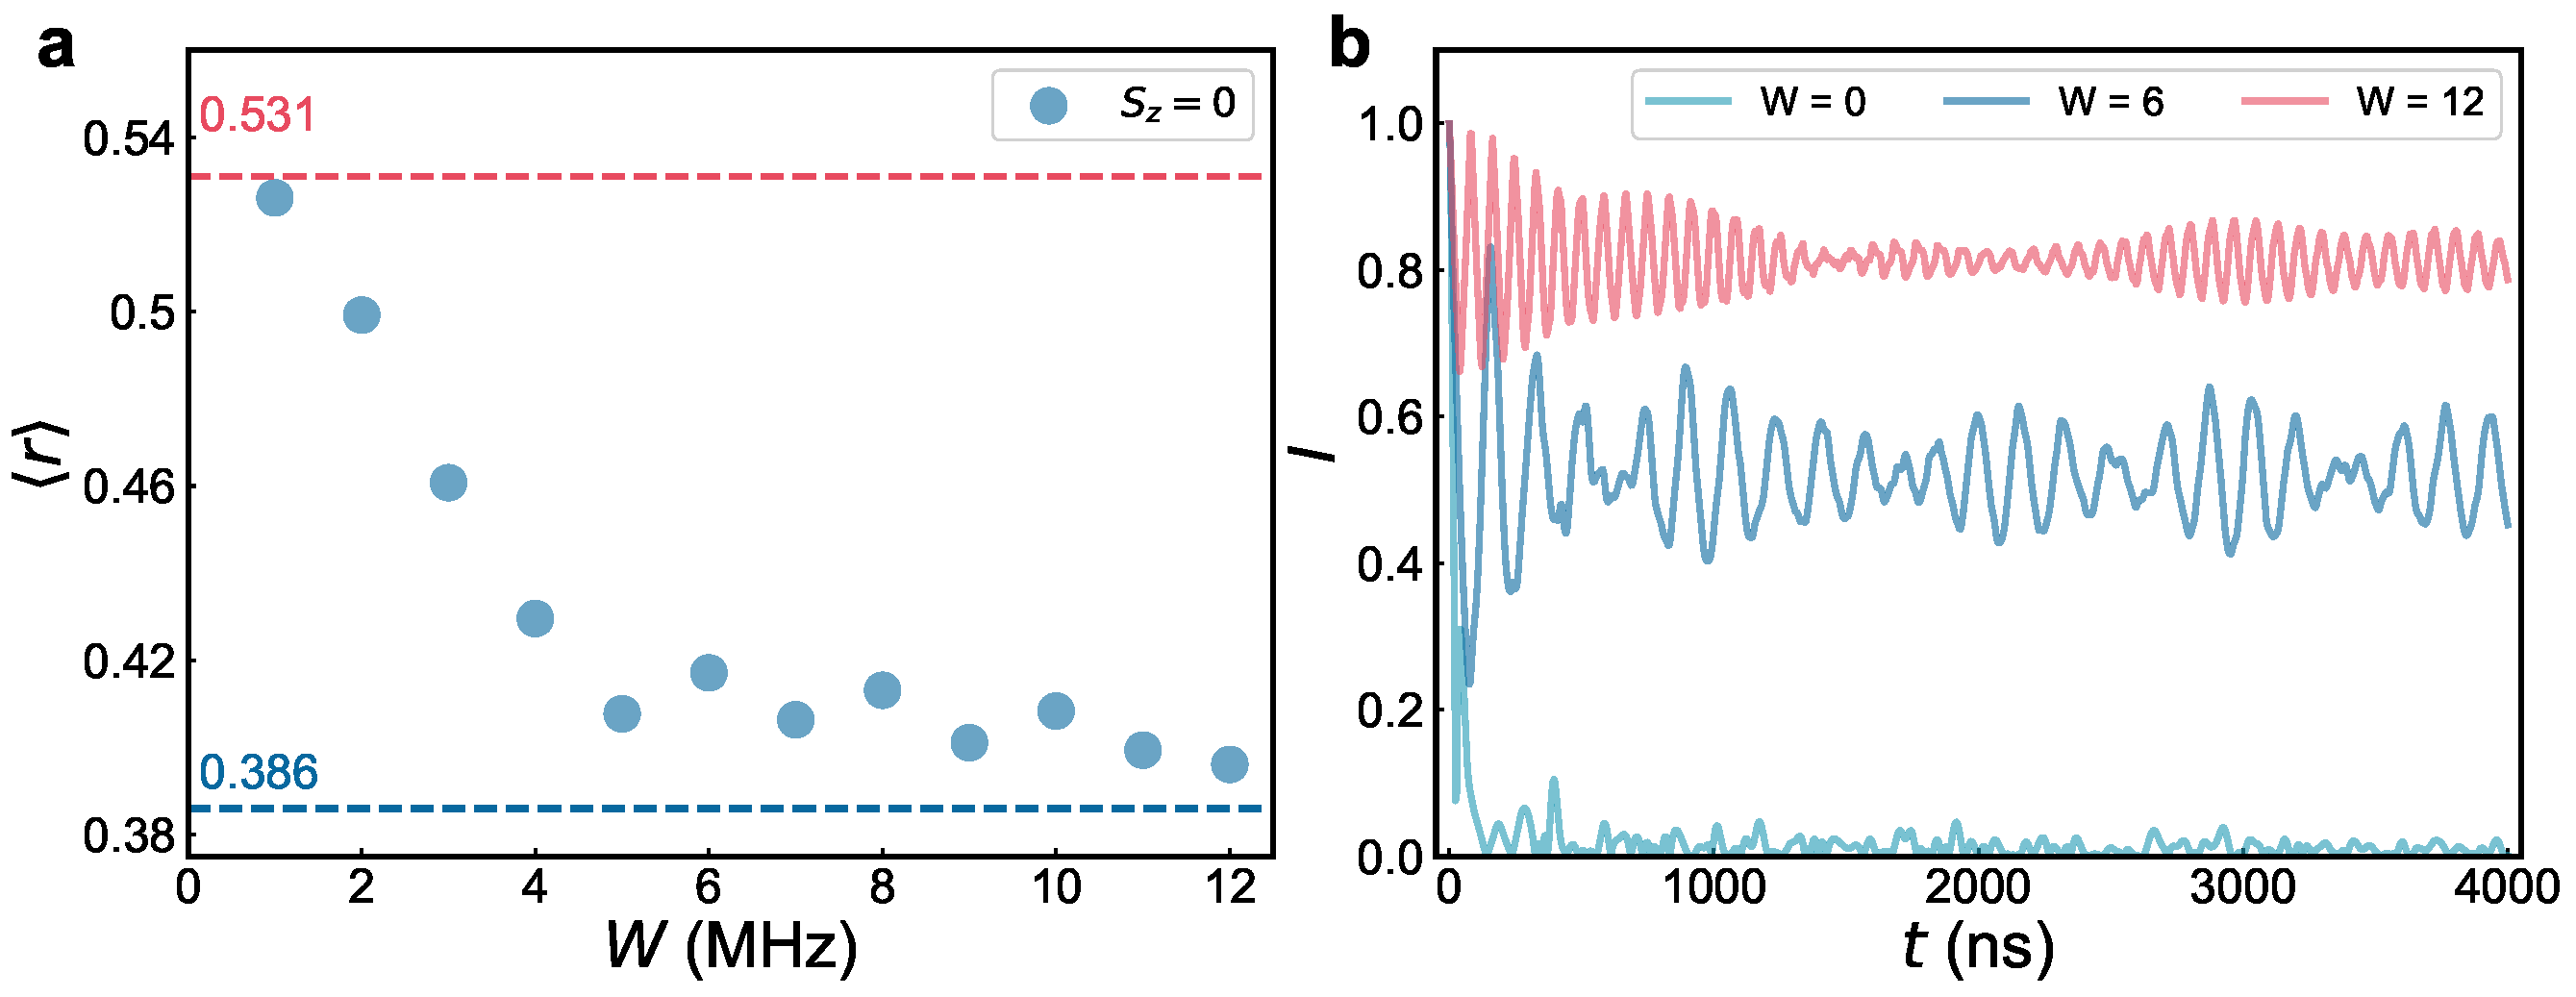
\includegraphics[width=0.95\textwidth]{SupFigS12.pdf}
    \caption{
        \textbf{线性势下遍历性破缺的指标。}
        (a) $S_z=0$子空间中平均能级间距比$\langle r\rangle$与势强度$W$的关系。
        在大$W$处$\langle r\rangle$接近$0.386$标志着遍历性破缺的开始,与泊松统计一致。
        (b) 对于$W=6,12$ MHz的不平衡动力学显示出围绕有限值的持续振荡,提供了非遍历行为的补充证据。
    }
    \label{fig:ergodicity_breaking}
\end{figure}

\begin{figure}[H]
    \centering
    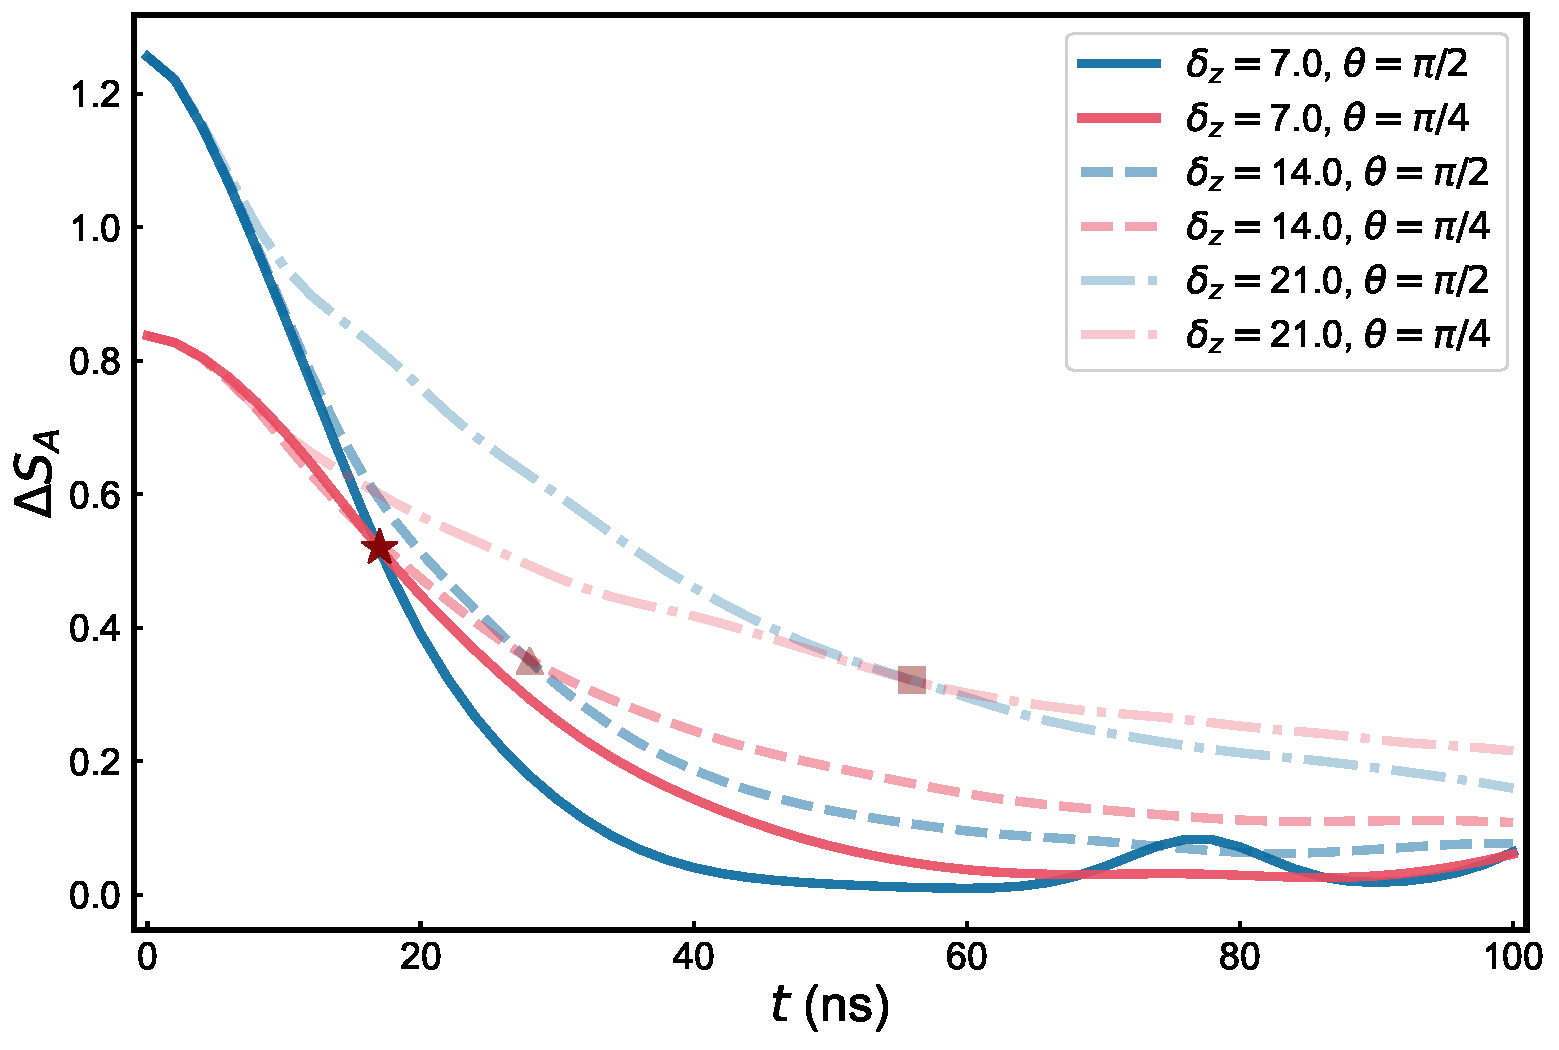
\includegraphics[width=0.7\textwidth]{SupFigS13.pdf}
    \caption{
        \textbf{倾斜铁磁态在不同无序强度下的纠缠不对称性动力学。}
        该图展示了在中间耦合区间($r \approx 1$)下,倾斜铁磁态在不同无序强度$\delta_z$时的EA动力学行为。
        (a) 弱无序条件($\delta_z = 7$)下,EA交叉现象清晰可见,量子Mpemba效应保持明显。
        (b) 中等无序条件($\delta_z = 14$)下,虽然动力学振荡被抑制,但特征性的EA交叉仍然存在。
        (c) 强无序条件($\delta_z = 21$)下,对称性恢复过程显著减缓,但EA交叉现象依然可观测。
        这些结果表明,基于倾斜铁磁态的量子Mpemba效应在宽范围的无序强度下都具有良好的鲁棒性,
        即使在破坏集体行为和周期性复兴的强无序条件下,其核心特征仍然得以保持。
    }
    \label{fig:disorder_strength_EA}
\end{figure}

对于倾斜铁磁态,在无无序情况下QME持续存在,并在研究的无序强度$h_i\in[-\delta_z,\delta_z]\bar{g}$下表现出卓越的鲁棒性,其中$\delta_z=7,14,21$。如图所示,特征性的EA交叉尽管存在强无序仍然持续。

\subsection{退相干效应与模拟方法}

实验退相干影响EA动力学。先前的研究证明,虽然退相干加速对称性恢复,但它本身不能产生QME。至关重要的是,我们的结果——连同参考文献[60]中的结果——揭示了QME在现实退相干条件下的鲁棒性。

EA动力学的精确模拟需要通过Lindblad主方程纳入退相干。传统的Liouville算符方法面临计算限制,对于$N$量子比特系统,内存需求按$\mathcal{O}(2^{4N})$缩放,对于大系统变得禁止性昂贵。

量子轨迹方法提供了一种有效的替代方案,以计算时间交换内存资源。这种技术通过无穷小时间步长$dt$模拟连续量子测量。在每个步骤,测量结果为:
\[
dy = \langle X\rangle dt + \frac{dW}{\sqrt{8\kappa}}
\]
其中$X$是测量算符,$dW$表示满足以下条件的Wiener噪声:
\[
\mathbb{E}[dW] = 0, \quad \text{Var}[dW] = dt
\]

状态演化遵循随机薛定谔方程:
\[
d|\psi\rangle = \left[-iHdt - \kappa(X-\langle X\rangle)^2 dt + \sqrt{2\kappa}(X-\langle X\rangle)dW\right]|\psi(t)\rangle
\]

等价地,密度矩阵根据随机主方程演化:
\[
d\rho = -i[H,\rho]dt - \kappa[X,[X,\rho]]dt + \sqrt{2\kappa}\left(X\rho + \rho X - 2\langle X\rangle\rho\right)dW
\]

值得注意的是,对$M$条轨迹的平均恢复了精确的Lindblad动力学:
\[
d\tilde{\rho} = -i[H,\tilde{\rho}]dt - \kappa[X,[X,\tilde{\rho}]]dt
\]
其中$\tilde{\rho}(t) = \frac{1}{M}\sum_{i=1}^{M}\rho_i(t)$。这种等价性将内存需求从$\mathcal{O}(2^{4N})$状态向量模拟转换为$\mathcal{O}(2^{N})$状态向量模拟,代价是$M/dt$时间步长,有效地将内存约束转换为计算时间。

量子轨迹方法的最佳实现需要平衡时间步长大小$dt$和轨迹计数$M$。我们针对$N=10$量子比特系统验证了这种方法与精确Lindblad解的比较,如图所示,证明了随着轨迹计数$M$增加,结果收敛到精确Lindblad解。图进一步显示了在实验参数下,随着$M$增加,EA动力学的收敛。这些结果确认,在足够的轨迹和适当的时间离散化下,量子轨迹方法可靠地近似了大尺度量子系统的Lindblad演化。主手稿中的模拟结果通过量子轨迹方法获得,使用时间步长$dt=0.15$和$M=100$条轨迹。

\begin{figure}[H]
    \centering
    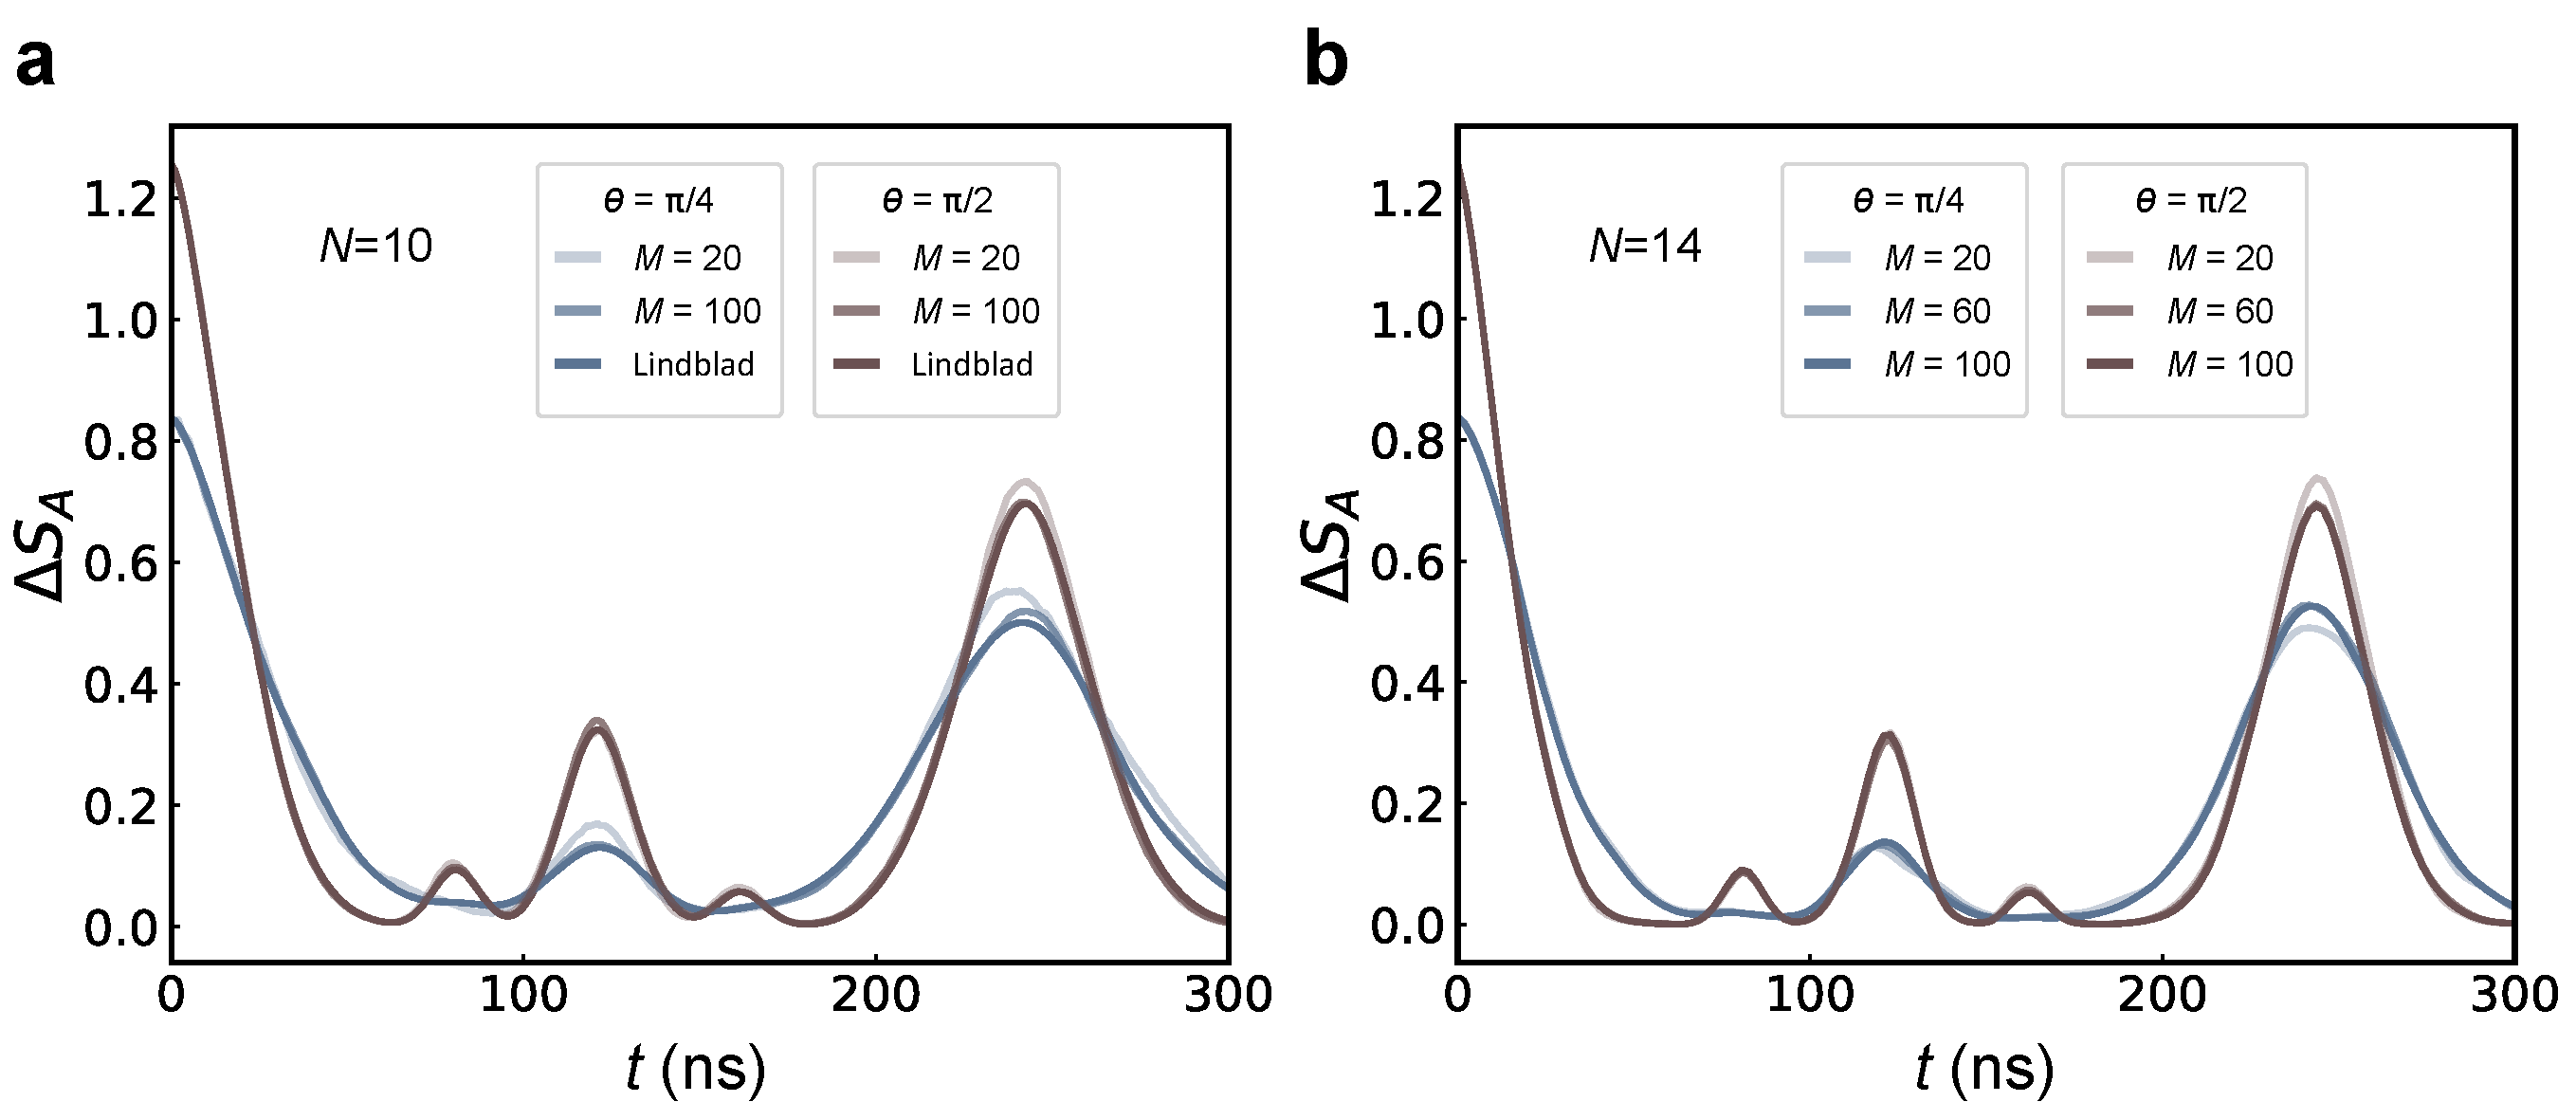
\includegraphics[width=0.95\textwidth]{SupFigS14.pdf}
    \caption{
        \textbf{使用量子轨迹方法验证倾斜铁磁态的EA动力学。}
        (a) 对于小系统($N=10$),随着轨迹计数$M$增加,结果接近从Lindblad方程的精确解获得的结果。
        (b) 随着轨迹计数$M$增加,结果逐渐收敛。
        所有结果通过量子轨迹方法获得。
    }
    \label{fig:quantum_trajectory_verification}
\end{figure}


\section{主方程、Lindblad、蒙特卡洛与量子轨迹的概念辨析}

\subsection{详细概念辨析}

\begin{table}[H]
\centering
\caption{主方程、Lindblad、蒙特卡洛与量子轨迹的概念辨析}
\begin{tabular}{|p{0.22\textwidth}|p{0.2\textwidth}|p{0.25\textwidth}|p{0.25\textwidth}|}
\hline
\textbf{概念} & \textbf{定义层次} & \textbf{核心思想} & \textbf{在论文中的应用} \\
\hline
\textbf{主方程} & \textbf{理论框架} & 描述系统\textbf{密度矩阵}随时间演化的微分方程 & 开放量子系统动力学的基本描述框架 \\
\hline
\textbf{Lindblad} & \textbf{具体形式} & 主方程的\textbf{特定形式},保证完全正定性和迹守恒 & 描述包含退相干的系统演化 \\
\hline
\textbf{蒙特卡洛} & \textbf{算法类型} & 通过\textbf{随机采样}来估计复杂问题的数值方法 & 量子轨迹方法的数学基础 \\
\hline
\textbf{量子轨迹} & \textbf{具体算法} & 通过模拟多条\textbf{随机状态演化路径}来重构密度矩阵 & 论文中用于高效模拟多体系统动力学的实际算法 \\
\hline
\end{tabular}
\label{tab:concept_comparison}
\end{table}

\subsection{深入理论解释}

\subsubsection{主方程 - 理论框架}

主方程是描述开放量子系统动力学的一般理论框架:
\[
\frac{d\rho}{dt} = \mathcal{L}[\rho]
\]
其中:
\begin{itemize}
    \item \textbf{定位}:理论框架
    \item \textbf{目标}:描述密度矩阵 $\rho$ 的演化
    \item \textbf{特点}:可以是各种形式,不一定是完全正定的
\end{itemize}

\subsubsection{Lindblad 主方程 - 具体实现}

Lindblad 主方程是主方程的一种特定形式:
\[
\frac{d\rho}{dt} = -i[H,\rho] + \sum_k \left(L_k\rho L_k^\dagger - \frac{1}{2}\{L_k^\dagger L_k, \rho\}\right)
\]
其中:
\begin{itemize}
    \item $H$:系统哈密顿量
    \item $L_k$:Lindblad 算符(跳变算符)
    \item \textbf{要求}:保证演化完全正定、迹守恒
    \item \textbf{优势}:物理上合理的耗散描述
\end{itemize}

\subsubsection{量子轨迹方法 - 计算算法}

\textcolor{magenta}{量子轨迹方法通过随机演化状态向量来近似密度矩阵演化:}
\[
|\psi(t)\rangle \xrightarrow{\text{随机演化}} |\psi(t+dt)\rangle
\]
最终密度矩阵为:
\[
\tilde{\rho}(t) = \frac{1}{M}\sum_{i=1}^{M} |\psi_i(t)\rangle\langle\psi_i(t)|
\]
其中:
\begin{itemize}
    \item \textbf{定位}:数值算法
    \item \textbf{原理}:\textcolor{magenta}{用大量随机轨迹的平均来近似密度矩阵演化}
    \item \textbf{优势}:内存效率高,适合大系统
\end{itemize}

\subsubsection{蒙特卡洛 - 数学基础}

\begin{itemize}
    \item \textbf{定位}:算法思想
    \item \textbf{原理}:\textcolor{magenta}{用随机性解决确定性问题的统计方法}
    \item \textbf{在量子轨迹中}:随机选择量子跳跃的时间和类型
\end{itemize}

\subsection{在量子Mpemba效应研究中的应用}

\subsubsection{计算挑战与解决方案}

在论文的 Supplementary Note 4 中,面临的主要计算挑战是:

\textbf{问题}:直接求解 Lindblad 方程的内存需求为 $\mathcal{O}(2^{4N})$,对于 $N=14$ 的量子比特系统变得不可行。

\textbf{解决方案}:采用量子轨迹方法
\begin{itemize}
    \item 内存需求:$\mathcal{O}(2^{N})$ 状态向量
    \item 计算代价:$M/dt$ 时间步长
    \item 实现方式:$\tilde{\rho}(t) = \frac{1}{M}\sum_{i=1}^{M} |\psi_i(t)\rangle\langle\psi_i(t)|$
\end{itemize}

% \subsubsection{计算流程}
% \begin{figure}[H]
%     \centering
%     \begin{tikzpicture}
%         \node (lindblad) [rectangle, draw] {Lindblad主方程\\(理论模型)};
%         \node (trajectory) [rectangle, draw, below of=lindblad] {量子轨迹方法\\(求解算法)};
%         \node (montecarlo) [rectangle, draw, below of=trajectory] {蒙特卡洛采样\\(数学基础)};
%         \node (results) [rectangle, draw, below of=montecarlo] {数值结果\\(EA动力学)};
        
%         \draw[->] (lindblad) -- (trajectory);
%         \draw[->] (trajectory) -- (montecarlo);
%         \draw[->] (montecarlo) -- (results);
%     \end{tikzpicture}
%     \caption{量子轨迹方法计算流程图}
%     \label{fig:computation_flow}
% \end{figure}

\subsection{重要理论区分}

\subsubsection{理论与算法的区分}

\begin{itemize}
    \item \textbf{Lindblad}:描述系统\textbf{应该怎样演化}(物理理论)
    \item \textbf{量子轨迹}:\textbf{如何计算}这种演化(数值算法)
\end{itemize}

\subsubsection{密度矩阵与状态向量的区分}

\begin{itemize}
    \item \textbf{主方程}:直接处理密度矩阵 $\rho$($N$量子比特:$2^N \times 2^N$ 矩阵)
    \item \textbf{量子轨迹}:处理状态向量 $|\psi\rangle$($N$量子比特:$2^N$ 向量)
\end{itemize}

\subsection{总结}

\textbf{核心关系总结}:
\begin{itemize}
    \item \textbf{主方程}是``我们要解什么''(理论框架)
    \item \textbf{Lindblad}是``方程的特定写法''(具体形式)  
    \item \textbf{蒙特卡洛}是``用随机抽样的思想''(算法基础)
    \item \textbf{量子轨迹}是``具体怎么算的算法''(数值实现)
\end{itemize}

在量子Mpemba效应的研究中,使用\textbf{量子轨迹方法}(基于蒙特卡洛思想)来数值求解\textbf{Lindblad主方程},从而避免了直接求解主方程时巨大的内存需求,使得模拟14量子比特系统的纠缠不对称性(EA)动力学成为可能。这种方法的成功应用是论文能够系统研究多体非平衡量子动力学的重要技术基础。



\end{document}